\documentclass[fontset=none]{Notes}

\makeatletter
\DeclareRobustCommand{\em}{%
  \@nomath\em \if b\expandafter\@car\f@series\@nil
  \normalfont \else \bfseries \fi}
\makeatother

\usepackage{tikz-cd,wrapstuff}
\usepackage{siunitx,tikz,nicematrix}
\usetikzlibrary{matrix,calc}
\usetikzlibrary{intersections}
\usetikzlibrary{arrows.meta}
\usetikzlibrary{decorations.markings}

\ProvidesFile{font.def}

\setCJKmainfont{Source Han Serif SC}[
  UprightFont=*-Regular,
  BoldFont=*-Bold,
  ItalicFont=HYKaiTi S,
  ItalicFeatures={Scale=1.1}
]
\newCJKfontfamily[zhsong]\songti{Source Han Serif SC}[
  UprightFont=*-Regular,
  BoldFont=*-Bold,
  ItalicFont=HYKaiTi S,
  ItalicFeatures={Scale=1.1}
]
\setCJKsansfont{Source Han Sans SC}[
  UprightFont=*-Regular,
  BoldFont=*-Bold
]
\newCJKfontfamily[zhhei]\heiti{Source Han Sans SC}[
  UprightFont=*-Regular,
  BoldFont=*-Bold
]
\setCJKmonofont{HYFangSong S}[
  BoldFont=*,
  ItalicFont=*,
  BoldItalicFont=*
]
\newCJKfontfamily[zhfs]\fangsong{HYFangSong S}[
  BoldFont=*,
  ItalicFont=*,
  BoldItalicFont=*
]
\newCJKfontfamily[zhkai]\kaishu{HYKaiTi S}[
  BoldFont=*,
  ItalicFont=*,
  BoldItalicFont=*
]

\setmainfont{texgyretermes}[
  Extension=.otf,
  UprightFont=*-regular,
  BoldFont=*-bold,
  ItalicFont=*-italic,
  BoldItalicFont=*-bolditalic,
  SlantedFont=*-italic
]
%\setmathrm{texgyretermes}[
%  Extension=.otf,
%  UprightFont=*-regular,
%  BoldFont=*-bold,
%  ItalicFont=*-italic,
%  BoldItalicFont=*-bolditalic,
%  SlantedFont=*-italic
%]
\setsansfont{Cantarell}[
  UprightFont=* Regular,
  ItalicFont=* Italic,
  BoldFont=* Bold,
  BoldItalicFont=* Bold Italic,
  SmallCapsFont=Alegreya Sans SC
]
\setmonofont{Ubuntu Mono}[
  UprightFont=*,
  ItalicFont=* Italic,
  BoldFont=* Bold,
  BoldItalicFont=* Bold Italic
]
%\setmathfont{texgyretermes-math.otf}
%\setmathfont[range={\mathcal,\mathbfcal,\mathfrak},StylisticSet=1]{XITSMath-Regular.otf}
%\setmathfont[range={\mathbb}]{KpMath-Sans.otf}



\usepackage[subscriptcorrection,nofontinfo,mtpbb,mtpfrak]{mtpro2}
\usepackage[normal]{fixdif}

\tikzcdset{
  arrow style=tikz,
  diagrams={>={Straight Barb[scale=0.8]}}
}

\tikzset{
  every picture/.style={
    thick,
    >={Latex[width=6pt, length=8pt]}
  },
  point/.style={
    circle, fill, minimum width=5pt,
    inner sep=0pt
  },
  straight arrow/.style={
    Straight Barb[scale=0.8]
  }
}

\allowdisplaybreaks[1]

\newlength{\mymathln}
\newcommand{\aligninside}[2]{
  \settowidth{\mymathln}{#2}
  \mathmakebox[\mymathln]{#1}
}

\DeclareMathOperator\Spec{Spec}
\DeclareMathOperator\im{im}
\DeclareMathOperator\sgn{sgn}
\DeclareMathOperator\rad{rad}
\DeclareMathOperator\Alt{Alt}
\DeclareMathOperator\Max{Max}
\DeclareMathOperator\card{card}
\DeclareMathOperator\GL{GL}
\DeclareMathOperator\Orth{O}
\DeclareMathOperator\SO{SO}
\DeclareMathOperator\SU{SU}
\DeclareMathOperator\cls{cls}
\DeclareMathOperator\Lie{Lie}
\DeclareMathOperator\End{End}
\DeclareMathOperator\Int{Int}
\DeclareMathOperator\Sym{Sym}
\DeclareMathOperator\tr{tr}
\DeclareMathOperator\Hom{Hom}
\DeclareMathOperator\supp{supp}
\DeclareMathOperator\Id{Id}
\DeclareMathOperator\rk{rank}
\DeclareMathOperator\grad{grad}
\DeclareMathOperator\rank{rank}
\DeclareMathOperator\Euc{E}
\DeclareMathOperator\ob{ob}
\DeclareMathOperator\diam{diam}
\DeclareMathOperator\rel{rel}
\newcommand{\LL}{{\mathrm{L}}}

\newcommand{\norm}[1]{\left\lVert#1\right\rVert}
\newcommand{\mat}[1]{\mathbold{#1}}
\newcommand{\cat}[1]{\mathsf{#1}}
\newcommand{\uline}{\underline{\hphantom{X}}}
\newcommand{\abs}[1]{\left|#1\right|}
\newcommand{\lie}[1]{\mathfrak{#1}}
\newcommand{\inn}[1]{\left\langle #1\right\rangle}
\newcommand{\partI}{\partial I}
\newcommand{\relhomo}{\rel\partI}

\usepackage{enumitem}

\setlist[enumerate]{nosep}

%\DeclareMathAlphabet\mathcal{OMS}{cmsy}{m}{n}

\newlength\stextwidth
\newcommand\makesamewidth[3][c]{%
  \settowidth{\stextwidth}{#2}%
  \makebox[\stextwidth][#1]{#3}%
}



\begin{document}

\frontmatter

\tableofcontents

\mainmatter

\setcounter{chapter}{-1}

\chapter{导论}

\section{Brouwer 不动点定理}

我们首先概述 Brouwer 不动点定理的证明:如果 $f:D^n\to D^n$ 是连续映射,
那么存在 $x\in D^n$ 使得 $f(x)=x$。当 $n=1$ 的时候,这个定理是容易证明的,
此时 $D^1$ 是闭区间 $[-1,1]$,我们在正方形 $D^1\times D^1$ 内观察
$f$ 的图像。
\begin{figure}[h]
  \centering
  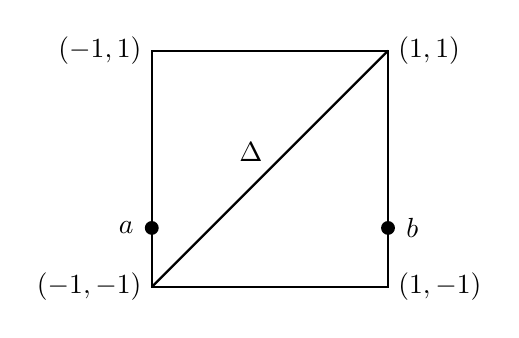
\begin{tikzpicture}[
      scale=1.5
    ]
    \draw (-1,-1) coordinate (v1) rectangle (1,1) coordinate (v2);
    \draw (v1) -- node[midway,above left=-1pt] {$\Delta$} (v2);
    \node [point,label=180:$a$] at ([yshift=0.5cm]v1) {};
    \node [point,label=0:$b$] at ([yshift=0.5cm]v1-|v2) {};
    \node [left] at (v1) {$(-1,-1)$};
    \node [left] at (v1|-v2) {$(-1,1)$};
    \node [right] at (v2) {$(1,1)$};
    \node [right] at (v2|-v1) {$(1,-1)$};
  \end{tikzpicture}
\end{figure}

\begin{theorem}
  每个连续映射 $f:D^1\to D^1$ 都有一个不动点。
\end{theorem}
\begin{proof}
  设 $f(-1)=a$ 以及 $f(1)=b$。要是 $f(-1)=-1$ 或者 $f(1)=1$,那么
  这就已经存在不动点,所以我们假设 $f(-1)=a>-1$ 以及 $f(1)=b<1$。
  设 $G$ 是 $f$ 的图像,$\Delta$ 是恒等映射的图像(对角线),我们需要证明
  $G\cap\Delta\neq \emptyset$。想法是利用连通性说明 $D^1\times D^1$
  中从 $a$ 到 $b$ 的道路必须与 $\Delta$ 相交。$f$ 连续表明 
  $G=\{(x,f(x))\,|\, x\in D^1\}$ 是连通的。定义 $A=\{(x,f(x))\,|\, f(x)>x\}$
  和 $B=\{(x,f(x))\,|\, f(x)<x\}$,注意到 $a\in A$ 和 $b\in B$。
  假设 $G\cap \Delta=\emptyset$,那么这表明 $G=A\cup B$ 是无交并,而
  $A,B$ 都是 $G$ 中的非空开集,与 $G$ 连通矛盾。
\end{proof}

不幸的是,当 $n>1$ 的时候没有人知道如何应用这个初等的拓扑证明,所以
必须引入新的思想。通过代数拓扑可以给出 Brouwer 不动点定理的一个证明。
我们最终将证明,对于每个 $n\geq 0$,存在一个\emph{同调函子} $H_n$
使得:对于每个拓扑空间 $X$,都给出一个交换群 $H_n(X)$;
对于每个连续映射 $f:X\to Y$,都给出一个同态 $H_n(f):H_n(X)\to H_n(Y)$
使得
\begin{equation}
  H_n(g\circ f)=H_n(g)\circ H_n(f)
\end{equation}
以及 $H_n(1_X)$ 是 $H_n(X)$ 上的恒等映射;此外还有
\begin{alignat}{2}
  &H_n(D^{n+1})=0 &\quad &\text{for all $n\geq 1$},\\
  &H_n(\mathbb{S}^{n})\neq 0 &&\text{for all $n\geq 1$}
  \label{eq:H_n(S^n)}.
\end{alignat}
使用 $H_n$ 的这些性质,我们现在可以证明 Brouwer 不动点定理。

\begin{definition}
  拓扑空间 $Y$ 的一个子空间 $X$ 被称为 $Y$ 的一个\emph{收缩},如果
  存在连续映射 $r:Y\to X$ 使得对于所有的 $x\in X$ 有 $r(x)=x$。
  这样的 $r$ 被称为一个\emph{收缩映射}。
\end{definition}

\begin{remark}
  (1)
  我们可以使用映射的语言重新叙述收缩映射的定义。如果 $\iota:X\hookrightarrow Y$
  是包含映射,那么连续映射 $r:Y\to X$ 是收缩映射当且仅当 $\iota$ 是 $r$ 的右逆,
  即 $r\circ\iota=1_X$。

  (2) 对于交换群来说,可以证明 $G$ 的子群 $H$ 是 $G$ 的收缩当且仅当 
  $H$ 是 $G$ 的一个直和项,也即存在 $G$ 的子群 $K$ 使得 $G=H\oplus K$。
\end{remark}

\begin{lemma}\label{lemma:S^n is not retract of D^n+1}
  如果 $n\geq 0$,那么 $\mathbb{S}^n$ 不是 $D^{n+1}$ 的收缩。
\end{lemma}
\begin{proof}
  假设存在收缩 $r:D^{n+1}\to \mathbb{S}^n$,那么我们有交换图
  \[
    \begin{tikzcd}[column sep=1.8em]
      & D^{n+1}\arrow[dr,"r"] & \\
      \mathbb{S}^n\arrow[ur,"\iota"]\arrow[rr,"1"'] & & \mathbb{S}^n ,
    \end{tikzcd}
  \]
  利用函子 $H_n$,给出了交换群的一个交换图
  \[
    \begin{tikzcd}[column sep=1em]
      & H_n(D^{n+1})\arrow[dr,"H_n(r)"] & \\
      H_n(\mathbb{S}^n)\arrow[ur,"H_n(\iota)"]\arrow[rr,"H_n(1)"'] & & 
      H_n(\mathbb{S}^n ),
    \end{tikzcd}
  \]
  由于 $H_n(D^{n+1})=0$,所以 $H_n(1)=H_n(\iota)\circ H_n(r)=0$,但是
  $H_n(1)$ 又必须是恒等映射,所以 $H_n(\mathbb{S}^n)=0$,这
  和 \eqref{eq:H_n(S^n)} 矛盾。
\end{proof}

注意到同调函子 $H_n$ 将拓扑问题转化为了代数问题。此外,
\autoref{lemma:S^n is not retract of D^n+1} 在 $n=0$ 的时候有很简单的证明,
此时收缩 $r:D^1\to \mathbb{S}^0=\{\pm 1\}$ 将连通空间映射到不连通空间,
这是不可能的。

\begin{theorem}[Brouwer]\label{thm:Brouwer}
  如果 $f:D^n\to D^n$ 是连续映射,那么 $f$ 有一个不动点。
\end{theorem}
\begin{proof}
  假设对于所有的 $x\in D^n$ 都有 $f(x)\neq x$,此时 $x$ 和 $f(x)$
  确定了一条直线。定义 $g:D^n\to \mathbb{S}^{n-1}$ 将 $x$ 映射
  为 $f(x)$ 到 $x$ 的射线与 $\mathbb{S}^{n-1}$ 的交点。
  \begin{center}
    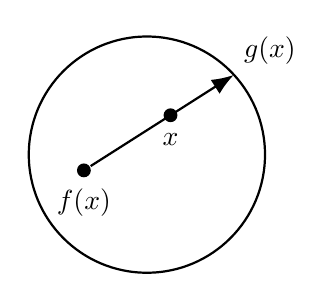
\begin{tikzpicture}
      \draw [name path=circ] (0,0) circle (1.5);
      \node [point,label=-90:$x$] (x) at (0.3,0.5) {}; 
      \node [point,label=-90:$f(x)$] (fx) at (-0.8,-0.2) {};
      \path [name path=line] (fx) -- ($(fx)!2!(x)$);
      \draw [->,name intersections={of=circ and line, by={gx}}]
        (fx) -- (gx) node [above right] {$g(x)$};
    \end{tikzpicture}
  \end{center}
  显然
  $x\in \mathbb{S}^{n-1}$ 表明 $g(x)=x$。利用坐标不难计算得 $g$ 
  是连续映射。
  这样 $g$ 就构成了一个收缩映射,与前面的引理矛盾。
\end{proof}

\begin{problem}{}{}
令 $H$ 是交换群 $G$ 的子群。如果存在同态 $r:G\to H$ 使得
对任意 $x\in H$ 有 $r(x)=x$,那么 $G=H\oplus \ker r$。  
\end{problem}
\begin{proof}
  任取 $y\in G$,那么 $r(y-r(y))=r(y)-r(y)=0$,所以
  $y-r(y)\in\ker r$,所以 $y=r(y)+y-r(y)\in H+\ker r$,
  所以 $G=H+\ker r$。下面设 $x\in H\cap\ker r$,那么
  $x=r(x)=0$,所以 $H\cap\ker r=\emptyset$。
\end{proof}

\begin{problem}{}{}
  假设在 $n\geq 1$ 的时候已知
  \[
    H_i(\mathbb{S}^n)=\begin{cases}
      \mathbb{Z} & i=0,n,\\
      0 & \text{otherwise},
    \end{cases}
  \]
  证明 $\mathbb{S}^{n}$ 的赤道不是一个收缩。
\end{problem}
\begin{proof}
  设 $r:\mathbb{S}^n\to \mathbb{S}^{n-1}$ 是收缩映射。
  那么我们有交换图
  \[
    \begin{tikzcd}[column sep=1em]
      & H_i(\mathbb{S}^{n})\arrow[dr,"H_i(r)"] & \\
      H_i(\mathbb{S}^{n-1})\arrow[ur,"H_i(\iota)"]\arrow[rr,"H_i(1)"'] & & 
      H_i(\mathbb{S}^{n-1}),
    \end{tikzcd}
  \]
  取 $i=n-1$ 即可得出矛盾。
\end{proof}

\begin{problem}{}{}
  如果 $X$ 是同胚于 $D^n$ 的拓扑空间,那么连续映射
  $f:X\to X$ 有不动点。
\end{problem} 
\begin{proof}
  设 $\varphi:D^n\to X$ 是同胚映射,那么 $\varphi^{-1}\circ f\circ\varphi:D^n\to D^n$
  是连续映射且有不动点,即存在 $x$ 使得 $\varphi^{-1}(f(\varphi(x)))=x$,
  即 $f(\varphi(x))=\varphi(x)$,所以 $f$ 有不动点 $\varphi(x)$。
\end{proof}

\begin{problem}{}{}
  令 $f,g:I\to I\times I$ 是连续映射,并且 $f(0)=(a,0)$,
  $f(1)=(b,1)$,$g(0)=(0,c)$,$g(1)=(1,d)$。证明存在 $s,t\in I$
  使得 $f(s)=g(t)$,也就是说 $f$ 和 $g$ 的像集一定是相交的道路。
\end{problem}
\begin{proof}
  定义 $h:I\times I\to I\times I$ 为
\end{proof}


\section{范畴与函子}

\begin{definition}
  范畴 $\cat C$ 上的一个\emph{共轭}指的是所有态射的类 $\bigcup_{(A,B)}\Hom(A,B)$
  上的一个等价关系 $\sim$,满足:
  \begin{enumerate}
    \item 如果 $f\in\Hom(A,B)$ 以及 $f\sim f'$,那么 $f'\in\Hom(A,B)$;
    \item 如果 $f\sim f'$ 和 $g\sim g'$ 并且 $g\circ f$ 存在,那么
    $g\circ f\sim g'\circ f'$。
  \end{enumerate}
\end{definition}

\begin{theorem}
  令 $\cat C$ 是一个范畴附带一个共轭 $\sim$,令 $[f]$ 表示态射 $f$ 的等价类。
  定义 $\cat C'$ 为:
  \begin{align*}
    \ob \cat C'&=\ob \cat C;\\
    \Hom_{\cat C'}(A,B)&=\bigl\{[f]\bigm| f\in\Hom_{\cat C}(A,B)\bigr\};\\
    [g]\circ [f]&=[g\circ f].
  \end{align*}
  那么 $\cat C'$ 是一个范畴,称为 $\cat C'$ 的\emph{商范畴}。
\end{theorem}

\chapter{基本拓扑概念}

\section{同伦}

\begin{definition}
  如果 $X,Y$ 是拓扑空间,$f_0,f_1$ 是 $X$ 到 $Y$ 的连续映射,存在
  连续映射 $F:X\times I\to Y$ 使得
  \[
    F(x,0)=f_0(x),\quad F(x,1)=f_1(x),
  \]
  那么我们说 $F$ 是一个\emph{同伦映射},并且 $f_0$ \emph{同伦于}
  $f_1$,记为 $f_0\simeq f_1$。当需要强调同伦映射的时候,我们写作
  $F:f_0\simeq f_1$。
\end{definition}

如果记 $f_t:X\to Y$ 为 $f_t(s)=F(x,t)$,那么同伦 $F$ 给出了一族
从 $f_0$ 变形到 $f_1$ 的单参数连续映射。我们可以认为 $f_t$ 随着
时间 $t$ 变形。

\begin{lemma}[粘连引理]
  假设 $X$ 是有限个闭子集的并集:$X=\bigcup_{i=1}^n X_i$。
  如果对于某个空间 $Y$,存在一族连续映射 $f_i:X_i\to Y$,它们在
  重叠区域相同,即对于任意 $i,j$ 有 $f_i|_{X_i\cap X_j}=f_j|_{X_i\cap X_j}$,
  那么存在唯一的连续映射 $f:X\to Y$ 使得对于所有的 $i$ 有 $f|_{X_i}=f_i$。
\end{lemma}
\begin{proof}
  任取 $x\in X$,如果 $x\in X_i$,我们定义 $f(x)=f_i(x)$。
  由于 $f_i,f_j$ 在重叠区域相同,所以这个定义是良好的,我们只需要说明连续性。
  任取 $Y$ 的闭子集 $C$,那么
  \begin{equation*}
    f^{-1}(C)=\bigcup\bigl(X_i\cap f^{-1}(C)\bigr)=
    \bigcup f_i^{-1}(C),
  \end{equation*}
  由于 $f_i^{-1}(C)$ 是 $X_i$ 的闭集,所以是 $X$ 的闭集。
  所以 $f^{-1}(C)$ 是闭集,即 $f$ 是连续映射。
\end{proof}

粘合引理也可以有开集的版本,其证明是完全一致的。

\begin{lemma}{}{}
  假设 $X$ 是任意个开子集的并集:$X=\bigcup_i X_i$。
  如果对于某个空间 $Y$,存在一族连续映射 $f_i:X_i\to Y$,它们在
  重叠区域相同,
  那么存在唯一的连续映射 $f:X\to Y$ 使得对于所有的 $i$ 有 $f|_{X_i}=f_i$。
\end{lemma}

\begin{theorem}
  同伦是所有连续映射 $X\to Y$ 集合上的一个等价关系。
\end{theorem}
\begin{proof}
  \emph{自反性}。如果 $f:X\to Y$ 是连续映射,定义 $F(x,t)=f(x)$,
  显然 $F:f\simeq f$。

  \emph{对称性}。假设 $f\simeq g$,即存在连续映射 $F:X\times I\to Y$
  使得 $F(x,0)=f(x)$ 和 $F(x,1)=g(x)$。定义 $G:X\times I\to Y$
  为 $G(x,t)=F(x,1-t)$,那么 $G:g\simeq f$。

  \emph{传递性}。假设 $F:f\simeq g$ 以及 $G:g\simeq h$。定义
  $H:X\times I\to Y$ 为
  \[
    H(x,t)=\begin{cases}
      F(x,2t) & 0\leq t\leq \frac{1}{2},\\
      G(x,2t-1) & \frac{1}{2}\leq t\leq 1.
    \end{cases}
  \]
  根据粘合引理,所以 $H$ 连续,所以 $H:f\simeq h$。
\end{proof}

\begin{definition}
  如果 $f:X\to Y$ 是连续映射,我们说
  \[
    [f]=\{g:X\to Y\,|\, g\simeq f\}
  \]
  是 $f$ 的\emph{同伦类}。
\end{definition}

所有同伦类的集合记为 $[X,Y]$。

\begin{theorem}
  对于 $i=0,1$,令 $f_i:X\to Y$ 和 $g_i:Y\to Z$ 是连续映射。如果
  $f_0\simeq f_1$ 和 $g_0\simeq g_1$,那么 $g_0\circ f_0\simeq g_1\circ f_1$,
  即 $[g_0\circ f_0]=[g_1\circ f_1]$。
\end{theorem}
\begin{proof}
  令 $F:f_0\simeq f_1$ 和 $G:g_0\simeq g_1$ 是同伦映射。
  首先定义 $H:X\times I\to Z$ 为 $H(x,t)=G(f_0(x),t)$,
  那么 $H:g_0\circ f_0\simeq g_1\circ f_0$。
  另一方面,定义 $K:X\times I\to Z$ 为 $K(x,t)=g_1\circ F(x,t)$,
  那么 $K:g_1\circ f_0\simeq g_1\circ f_1$。
  根据同伦的传递性,就有 $g_1\circ f_1\simeq g_0\circ f_0$。
\end{proof}

\begin{corollary}
  同伦是拓扑范畴 $\cat{Top}$ 上的一个共轭。
\end{corollary}

这意味着存在一个商范畴,其对象是拓扑空间 $X$,态射集合 
$\Hom(X,Y)=[X,Y]$,复合为 $[g]\circ [f]=[g\circ f]$。

\begin{definition}
  上述商范畴被称为\emph{同伦范畴},记为 $\cat{hTop}$。
\end{definition}

我们即将构造的所有从 $\cat{Top}$ 到某个“代数”范畴 $\cat A$(例如 $\cat{Ab},\cat{Grp},\cat{Ring}$)
的函子 $T:\cat{Top}\to\cat{A}$ 都有性质使得 $f\simeq g$ 的时候有 $T(f)=T(g)$。
事实上,除开自然地希望将同伦映射视为等同的之外,这保证了通过 $T$
将拓扑问题转化为 $\cat A$ 中的代数问题是比原问题更加简单的。
此外,练习表明每个这样的函子都会给出一个函子 $\cat{hTop}\to\cat A$,
所以同伦范畴是相当基本的。

\begin{definition}
  一个连续映射 $f:X\to Y$ 被称为\emph{同伦等价},如果存在连续映射
  $g:Y\to X$ 使得 $g\circ f\simeq 1_X$ 和 $f\circ g\simeq 1_Y$。
  如果存在同伦等价 $f:X\to Y$,那么我们说空间 $X$ 和 $Y$
  有相同的\emph{同伦型}。
\end{definition}

显然,同胚的空间有相同的同伦型,但是反过来不对,我们将在后面看到。

下面的两个结果表明同伦可以和一些有趣的问题联系起来。

\begin{definition}
  令 $X,Y$ 是拓扑空间,$y_0\in Y$。$y_0$ 处的\emph{常值映射}
  指的是映射 $c:X\to Y$ 使得 $c(x)\equiv y_0$。
  对于连续映射 $f:X\to Y$,如果存在常值映射 $c$ 使得 $f\simeq c$,那么我们说 $f$ 是
  \emph{零伦的}。
\end{definition}

\begin{remark}
  我们将在后面看到 $\mathbb{C}\smallsetminus\{0\}$ 实质上是圆周
  $\mathbb{S}^1$,即 $\mathbb{C}\smallsetminus\{0\}$ 和 $\mathbb{S}^1$
  有相同的同伦型。
\end{remark}

拓扑学中一个常见的问题是将映射 $f:X\to Z$ 延拓到一个更大的空间 $Y$
中,即是否存在 $g:Y\to Z$ 使得有下面的交换图
\[
  \begin{tikzcd}[column sep=large,row sep=large]
    Y\arrow[dr,"g",dashrightarrow] & \\
    X\arrow[u,hook]\arrow[r,"f"'] & Z  .
  \end{tikzcd}
\]
同伦本身则引出了这样一个问题:如果 $f_0,f_1:X\to Z$ 且我们能够
延拓 $f_0\cup f_1:X\times\{0\}\cup X\times\{1\}\to Z$ 到
$X\times I$ 上,那么 $f_0\simeq f_1$。

\begin{theorem}\label{thm:S^n is nullhomotopic}
  令 $f:\mathbb{S}^n\to Y$ 是连续映射,下面的说法等价:
  \begin{enumerate}
    \item $f$ 是零伦的;
    \item $f$ 可以延拓为一个连续映射 $D^{n+1}\to Y$;
    \item 如果 $x_0\in \mathbb{S}^n$,$k:\mathbb{S}^n\to Y$
    是 $f(x_0)$ 处的常值映射,那么存在一个同伦 $F:f\simeq k$
    使得 $F(x_0,t)=f(x_0)$ 对于所有 $t\in I$ 成立。
  \end{enumerate}
\end{theorem}
\begin{proof}
  $(1)\Rightarrow(2)$ 假设 $F:f\simeq c$,其中 $c(x)=y_0$。定义
  $g:D^{n+1}\to Y$ 为
  \[
    g(x)=\begin{cases}
      y_0 & 0\leq \norm{x}\leq\frac{1}{2},\\
      F\bigl(x/\norm{x},2-2\norm{x}\bigr) & 
      \frac{1}{2}\leq\norm{x}\leq 1.
    \end{cases}
  \]
  根据粘合引理,$g$ 是连续映射。如果 $x\in \mathbb{S}^n$,那么
  $g(x)=F(x,0)=f(x)$,所以 $g$ 是 $f$ 的延拓。

  $(2)\Rightarrow(3)$ 假设 $g:D^{n+1}\to Y$ 是 $f$ 的延拓。定义
  $F:\mathbb{S}^{n}\times I\to Y$ 为 $F(x,t)=g((1-t)x+tx_0)$,
  显然 $F$ 是连续映射。由于 $F(x,0)=g(x)=f(x)$,$F(x,1)=g(x_0)=f(x_0)$,
  所以 $F:f\simeq k$。此外,$F(x_0,t)=g(x_0)=f(x_0)$。

  $(3)\Rightarrow (1)$ 显然。
\end{proof}

我们可以把这个定理和 \autoref{lemma:S^n is not retract of D^n+1} 对比。
如果 $Y=\mathbb{S}^n$ 以及 $f$ 是恒等映射,那么 \autoref{lemma:S^n is not retract of D^n+1}
表明 $f$ 不是零伦的,否则 $f$ 延拓为连续映射 $D^{n+1}\to \mathbb{S}^n$,这表明
$\mathbb{S}^n$ 是 $D^{n+1}$ 的收缩。

\section{凸性、可缩性以及锥体}

我们给上述证明中使用到的 $D^{n+1}$ 的一个性质起个名字。

\begin{definition}
  $\mathbb{R}^m$ 的子集 $X$ 被称为\emph{凸集},如果任取 $x,y\in X$,
  连接 $x,y$ 的线段都在 $X$ 中。换句话说,对于任意 $t\in I$,有
  $tx+(1-t)y\in X$。
\end{definition}

凸集的例子有很多,例如 $I^n$,$\mathbb{R}^n$,$D^n$ 和 $\Delta^n$
都是凸集。但是球面 $\mathbb{S}^n\subseteq \mathbb{R}^{n+1}$
不是凸集。

\begin{definition}
  空间 $X$ 被称为\emph{可缩的},如果 $1_X$ 是零伦的。
\end{definition}

\begin{theorem}
  每个凸集 $X$ 都是可缩的。
\end{theorem}
\begin{proof}
  任取 $x_0\in X$,定义 $c:X\to X$ 是常值映射 $c(x)=x_0$。
  令 $F:X\times I\to X$ 为 $F(x,t)=tx_0+(1-t)x$,那么 $F:1_X\simeq c$。
\end{proof}

半球面是可缩的但是不是凸集,所以上述定理的逆命题不正确。后面我们会
发现 \autoref{lemma:S^n is not retract of D^n+1} 实际上表明
$\mathbb{S}^n$ 是不可缩的。

\begin{problem}{}{}
  (1) 如果 $X\approx Y$ 且 $X$ 可缩,那么 $Y$ 也可缩。

  (2) 如果 $X,Y$ 是 Euclid 空间的子空间,$X\approx Y$ 且 $X$
  是凸集,证明 $Y$ 可能不是凸集。 
\end{problem}
\begin{proof}
  (1) 设 $c:X\to X$ 是常值映射 $c(x)=x_0$ 且 $1_X\simeq c$,
  $f:X\to Y$ 是同伦等价。设 $g:Y\to X$
  使得 $g\circ f\simeq 1_X$ 以及 $f\circ g\simeq 1_Y$。
  记 $k:Y\to Y$ 是常值映射 $k(y)=f(x_0)$,那么
  \[
    1_Y=1_Y \circ 1_Y\simeq 
    (f\circ g)\circ (f\circ g)\simeq f\circ 1_X\circ g
    \simeq f\circ c\circ g=k,
  \]
  所以 $Y$ 可缩。
\end{proof}

\begin{problem}{}{}
  令 $R:\mathbb{S}^1\to \mathbb{S}^1$ 表示旋转 $\alpha$ 弧度。证明
  $R\simeq 1_{\mathbb{S}^1}$。由此得出每个连续映射 $f:\mathbb{S}^1\to \mathbb{S}^1$
  都同伦于一个满足 $g(1)=1$ 的连续映射 $g:\mathbb{S}^1\to \mathbb{S}^1$。
\end{problem}
\begin{proof}
  即 $R(e^{i\theta})=e^{i(\theta+\alpha)}$。定义 $F:\mathbb{S}^1\times I\to \mathbb{S}^1$
  为 $F(e^{i\theta},t)=e^{i(\theta+t\alpha)}$,显然 $F$ 是连续映射,
  所以 $F:1_{\mathbb{S}^1}\simeq R$。任取连续映射 $f:\mathbb{S}^1\to \mathbb{S}^1$,
  设 $f(1)=e^{i\alpha}$,取 $R$ 为旋转 $-\alpha$,
  那么 $1_{\mathbb{S}^1}\circ f\simeq R\circ f$,此时 $g=R\circ f$
  满足 $g(1)=R(f(1))=1$。
\end{proof}

马上引入的锥体的构造将表明每个空间都可以嵌入到一个可缩空间中。
我们先回顾一下商空间的构造。

\begin{definition}
  令 $X$ 是拓扑空间,$\sim$ 是一个等价关系,那么有一个自然映射
  $\pi:X\to X/\sim$,即 $\pi(x)=[x]$。我们可以赋予 $X/\sim$ 一个\emph{商拓扑},
  即 $U\subseteq X/\sim$ 是开集当且仅当 $\pi^{-1}(U)$ 是 $X$
  的开集。
\end{definition}

有一种特殊的情况需要单独提及。如果 $A\subseteq X$,那么我们记 $X/A$
为划分 $\{A\}\cup \{\{x\}\,|\, x\in X \smallsetminus A\}$ 给出的商空间,
也就是说,这个构造将 $A$ 压缩为一点,而 $X \smallsetminus A$ 中的点保持不变。

\begin{definition}
  连续满射 $f:X\to Y$ 被称为\emph{商映射},如果 $U\subseteq Y$
  是开集当且仅当 $f^{-1}(U)$ 是 $X$ 的开集。
\end{definition}

\begin{example}
  \mbox{}
  \begin{enumerate}
    \item 自然映射 $\pi:X\to X/\sim$ 是商映射。
    \item 如果连续满射 $f:X\to Y$ 是开映射或者闭映射,那么 $f$
    是商映射。以开映射的情况为例,此时若 $U\subseteq Y$ 使得 $f^{-1}(U)$
    是开集,那么 $U=f(f^{-1}(U))$ 是 $Y$ 的开集。
    \item 如果连续映射 $f:X\to Y$ 有一个截面,即存在连续映射 $s:Y\to X$
    使得 $f\circ s=1_Y$,那么 $f$ 是商映射。首先 $s$ 是 $f$ 是右逆保证了
    $f$ 是满射。若 $U\subseteq Y$ 使得 $f^{-1}(U)$ 是开集,那么 
    $U=1_Y^{-1}(U)=(f\circ s)^{-1}(U)$ 是 $Y$ 的开集,所以 $f$
    是商映射。
  \end{enumerate}
\end{example}

\begin{theorem}
  令 $f:X\to Y$ 是连续满射。那么 $f$ 是商映射当且仅当:对于 
  任意空间 $Z$ 和映射 $g:Y\to Z$,$g$ 连续当且仅当 $g\circ f$ 连续。
  \[
    \begin{tikzcd}[column sep=large,row sep=large]
      X\arrow[d,"f"']\arrow[dr,"g\circ f"] & \\
      Y\arrow[r,"g"'] & Z.
    \end{tikzcd}
  \]
\end{theorem}
\begin{proof}
  假设 $f$ 是商映射。如果 $g$ 连续,显然 $g\circ f$ 连续。反之,如果
  $g\circ f$ 连续,任取 $Z$ 的开集 $V$,那么 
  $f^{-1}(g^{-1}(V))=(g\circ f)^{-1}(V)$ 是 $X$ 的开集,所以
  $g^{-1}(V)$ 是 $Y$ 的开集,所以 $g$ 连续。

  假设反过来成立。取 $Z=X/\sim$,$\sim$ 是映射 $f$ 的纤维诱导的 
  $X$ 的划分。那么我们有交换图
  \[
    \begin{tikzcd}[sep=large]
      X\arrow[d,"f"']\arrow[dr,"\pi"] &  \\
      Y & X/\sim\arrow[l,"\bar f"],
    \end{tikzcd}
  \]
  其中 $\bar f$ 是 $f$ 诱导的双射,此时 $\bar f^{-1}\circ f(x)=\pi(x)$,
  根据假设,$\bar f^{-1}$ 是连续映射,所以 $\bar f$ 是同胚,所以
  $f=\bar f\circ\pi$ 是商映射。
\end{proof}

\begin{corollary}
  令 $f:X\to Y$ 是商映射,$h:X\to Z$ 是连续映射并且在 $f$
  的每个纤维上是常值的,那么存在唯一的连续映射 $\bar h:Y\to Z$
  使得 $h=\bar h\circ f$,即有交换图
  \[
    \begin{tikzcd}[sep=large]
      X\arrow[d,"f"']\arrow[dr,"h"] &  \\
      Y\arrow[r,"\bar h"',dashed] & Z.
    \end{tikzcd}
  \]
  此外,$\bar h$ 是开(闭)映射当且仅当在
  $U$ 是 $X$ 的形如 $U=f^{-1}(f(U))$ 的开(闭)集时,
  $h(U)$ 是 $Z$ 的开(闭)集。
\end{corollary}
\begin{proof}
  要保证 $h=\bar h\circ f$,即任取 $x\in X$,有 $\bar h(f(x))=h(x)$。
  对于 $y=f(x)\in Y$,那么必须有 $\bar h(y)=\bar h(f(x))=h(x)$,
  $h$ 在 $f$ 的纤维上是常值的表明这样的 $\bar h$ 是良好定义的,所以
  $\bar h$ 唯一存在。$h=\bar h\circ f$ 连续表明 $\bar h$ 连续。

  以开映射为例。若 $\bar h$ 是开映射且 $U=f^{-1}(f(U))$ 是
  $X$ 的开集,那么 $h(U)=h(f^{-1}(f(U)))=\bar h(f(U))$,
  由于 $f^{-1}(f(U))=U$ 是 $X$ 的开集,所以 $f(U)$ 是 $Y$
  的开集,所以 $h(U)=\bar h(f(U))$ 是 $Z$ 的开集。
  反之,任取 $V\subseteq Y$ 是开集,那么 $f^{-1}(V)$ 是 $X$
  的开集且 $f^{-1}(V)=f^{-1}(f(f^{-1}(V)))$,
  根据假设,有 $h(f^{-1}(V))$ 是 $Z$ 的开集,
  于是 $\bar h(V)=\bar h(f(f^{-1}(V)))=h(f^{-1}(V))$
  是 $Z$ 的开集,即 $\bar h$ 是开映射。
\end{proof}

\begin{corollary}
  令 $X,Z$ 是拓扑空间,$h:X\to Z$ 是商映射,记 $X/\sim$ 是 $h$ 的纤维
  导出的商空间,那么 $X/\sim$ 同胚于 $Z$,同胚映射为 $\varphi:[x]\mapsto h(x)$。
\end{corollary}
\begin{proof}
  记自然映射 $\pi:X\to X/\sim$。由于 $h$ 在 $h$ 的纤维上是常值的,
  所以存在唯一的连续映射 $\varphi:X/\sim\,\to Z$ 使得 $h=\varphi\circ\pi$,
  即 $\varphi([x])=h(x)$。另一方面,$\pi$ 在 $h$ 的纤维上也是常值的,所以
  存在唯一的连续映射 $\psi:Z\to X/\sim$ 使得 $\pi=\psi\circ h$,
  所以 $h=\varphi\circ\pi=\varphi\circ\psi\circ h$,$h$
  是满射表明存在右逆,所以 $\varphi\circ\psi=1_Z$。
  同理可得 $\psi\circ\varphi=1_{X/\sim}$,所以 $\varphi$
  和 $\psi$ 互为连续逆映射,故 $\varphi$ 是同胚。
\end{proof}

\begin{problem}{}{}
  令 $f:X\to Y$ 是商映射,$g:Y\to Z$ 是连续满射,那么 $g$
  是商映射当且仅当 $g\circ f$ 是商映射。 
\end{problem}
\begin{proof}
  若 $g$ 是商映射,设 $W\in Z$ 使得 $(g\circ f)^{-1}(W)$
  是 $X$ 的开集,即 $f^{-1}(g^{-1}(W))$ 是 $X$ 的开集,
  所以 $g^{-1}(W)$ 是 $Y$ 的开集,所以 $W$ 是 $Z$
  的开集,所以 $g\circ f$ 是商映射。

  反之,若 $g\circ f$ 是商映射。设 $W\in Z$ 使得 $g^{-1}(W)$
  是开集,那么 $(g\circ f)^{-1}(W)=f^{-1}(g^{-1}(W))$
  是 $X$ 的开集,$g\circ f$ 是商映射表明 $W$ 是 $Z$ 的开集。
\end{proof}

\begin{problem}{}{}
  设 $X$ 和 $Y$ 是拓扑空间,分别有等价关系 $\sim$ 和 $\sim'$,
  $f:X\to Y$ 是保持关系的连续映射,即 $x\sim x'$ 能推出 $f(x)\sim' f(x')$。
  证明其诱导的 $\bar f:X/\sim\,\to Y/\sim'$ 是连续映射。此外,
  如果 $f$ 是商映射,那么 $\bar f$ 也是商映射。
\end{problem}
\begin{proof}
  记 $\pi:X\to X/\sim$ 和 $\pi':Y\to Y/\sim'$ 是自然映射。
  那么我们有交换图
  \[
    \begin{tikzcd}[sep=huge]
      X\arrow[r,"f"]\arrow[d,"\pi"'] & Y\arrow[d,"\pi'"]\\
      X/\sim\arrow[r,"\bar f"',dashed] & Y/\sim',
    \end{tikzcd}
  \] 
  其中 $\bar f([x])=[f(x)]$。$f$ 保持关系表明 $\bar f$ 是良好定义的。
  任取 $Y/\sim'$ 的开集 $V$,那么 
  \[
    \pi^{-1}(\bar f^{-1}(V))=(\bar f\circ\pi)^{-1}(V)=(\pi'\circ f)^{-1}(V)=f^{-1}(\pi'^{-1}(V))
  \]
  是 $X$ 的开集,所以 $\bar f^{-1}(V)$ 是 $X/\sim$ 的开集,
  故 $\bar f$ 是连续映射。如果 $f$ 是商映射,那么
  $\pi'\circ f$ 是商映射,再根据上一题,$\bar f$ 是商映射。
\end{proof}

\begin{definition}
  若 $X$ 是拓扑空间,定义 $X\times I$ 上的等价关系为 $(x,t)\sim (x',t')$
  当且仅当 $t=t'=1$。记 $(x,t)$ 所在的等价类为 $[x,t]$。
  我们说商空间 $X\times I/\sim$ 是 $X$ 上的\emph{锥体},记为 $CX$。
\end{definition}

实际上上面的定义表明 $CX$ 就是商空间 $X\times I/X\times\{1\}$。
点 $[x,1]\in CX$ 被称为\emph{顶点}。我们基本上相当于引入了一个新的不在
$x$ 中的点(顶点)$v$ 并且用线段连接了 $v$ 和 $X$ 中的每个点。

\begin{example}
  对于空间 $X$ 和 $Y$,任意连续映射 $f:X\times I\to Y$
  如果满足 $f(x,1)=y_0$,那么都诱导了连续映射 $\bar f:CX\to Y$
  为 $\bar f:[x,t]\mapsto f(x,t)$。特别地,令 $f:\mathbb{S}^{n}\times I\to D^{n+1}$
  是映射 $(u,t)\mapsto (1-t)u$,因为 $f(u,1)\equiv 0$,所以诱导连续映射
  $\bar f:C \mathbb{S}^n\to D^{n+1}$ 为 $[u,t]\mapsto (1-t)u$。实际上,
  $\bar f$ 还是一个同胚。我们说明 $f$ 是商映射即可,由于 $f$
  是紧空间到 Hausdorff 空间的连续映射,所以是闭映射,又因为 $f$
  是满射,所以 $f$ 是商映射。
\end{example}

\begin{theorem}
  对于每个空间 $X$,锥体 $CX$ 都是可缩的。
\end{theorem}
\begin{proof}
  定义 $F:CX\times I\to CX$ 为
  $F([x,t],s)=[x,s+(1-s)t]$ 即可。
\end{proof}

下面的结果表明可缩空间是 $\cat{hTop}$ 中最简单的对象。

\begin{theorem}
  空间 $X$ 和单点空间有相同的同伦型当且仅当 $X$ 是可缩的。
\end{theorem}
\begin{proof}
  设 $\{a\}$ 是单点空间。假设 $X$ 和 $\{a\}$ 有相同的同伦型,
  即存在连续映射 $f:X\to\{a\}$ 和连续映射 $g:\{a\}\to X$
  使得 $g\circ f\simeq 1_X$,由于 $g\circ f$ 显然是常值映射,
  所以 $X$ 是可缩的。

  假设 $X$ 是可缩的。设 $1_X\simeq c$,其中 $c:X\to X$ 是常值映射
  $c(x)=x_0$。令 $f:X\to \{x_0\}$ 和 $g:\{x_0\}\to X$,
  其中 $g(x_0)=x_0$。那么 $f\circ g=1_{\{x_0\}}$ 以及
  $g\circ f=c\simeq 1_X$,所以 $f:X\to \{x_0\}$ 是同伦等价。
\end{proof}

下面的定理表明可缩空间可能和单点集的行为类似,尤其是以同伦的角度来看的时候。

\begin{theorem}
  如果 $Y$ 可缩,那么任意 $X\to Y$ 的两个连续映射都是同伦的,
  等价地说,任意 $X\to Y$ 的连续映射都是零伦的。
\end{theorem}
\begin{proof}
  $Y$ 可缩表明 $1_Y\simeq c$,设 $c(y)=y_0$ 是常值映射。
  定义 $g:X\to Y$ 是常值映射 $g(x)=y_0$。任取连续映射 $f:X\to Y$,那么
  $f=1_Y\circ f\simeq c\circ f=g$,所以任意连续映射 $f$
  都同伦于 $g$。
\end{proof}
 
\section{道路和道路连通}

\begin{definition}
  $X$ 的一个\emph{道路}指的是一个连续映射 $f:I\to X$。如果 
  $f(0)=a$,$f(1)=b$,那么我们说 $f$ 是从 $a$ 到 $b$ 的道路。
\end{definition}

\begin{definition}
  如果对于任意 $a,b\in X$,都存在从 $a$ 到 $b$ 的道路,那么我们说
  $X$ 是\emph{道路连通}的。
\end{definition}

\begin{theorem}
  如果 $X$ 道路连通,那么 $X$ 连通。
\end{theorem}
\begin{proof}
  假设 $X$ 不连通,那么存在分离开集 $A,B$ 使得 $X=A\cup B$。
  取 $a\in A$ 和 $b\in B$,$X$ 道路连通表明存在从 $a$ 到 $b$
  的道路 $f:I\to X$,那么 $f(I)$ 是连通子集,但是
  $f(I)=\bigl(f(I)\cap A\bigr)\cup\bigl(f(I)\cap B\bigr)$,
  这与 $f(I)$ 连通矛盾。
\end{proof}

\begin{example}
  存在连通但是不道路连通的空间。\emph{拓扑学家的 sin 曲线}是一个
  经典的例子。定义空间 $X=A\cup G\subseteq \mathbb{R}^2$ 由两部分构成,
  其中 $A=\{(0,y)\,|\, -1\leq y\leq 1\}$,
  $G=\{(x,\sin(1/x))\,|\, 0<x\leq 1/2\pi\}$。
  不难证明 $X$ 是连通的,因为 $A\subseteq \wbar G$,
  所以 $X=\wbar G$ 是连通的。但是 $X$ 不是道路连通的。
  我们证明不存在从 $(0,0)$ 到 $(1/2\pi,0)$ 的道路。
  假设 $f:I\to X$ 是这样的道路,取 $t_0=\sup\{t\in I\,|\, f(t)\in A\}$,
  由于 $A$ 是 $X$ 的闭集,所以 $f^{-1}(A)\subseteq [0,t_0]$
  是闭集,而 $t_0$ 是 $f^{-1}(A)$ 的极限点,所以 $f(t_0)\in A$。
  同时,任意 $s\in (t_0,1]$ 都使得 $f(s)\in G$。那么我们可以选取
  递减趋于 $t_0$ 的一列 $\{s_n\}$ 使得 $f(s_n)=\bigl(2/(2n+1)\pi,(-1)^n\bigr)$,
  但是 $n\to\infty$ 的时候 $f(s_n)$ 并不收敛,这与 $f$ 的连续性矛盾。
\end{example}

\begin{problem}{}{null}
  (1) 空间 $X$ 是道路连通的当且仅当任意两个常值映射
    $X\to X$ 是同伦的。

  (2) 如果 $X$ 可缩,$Y$ 道路连通,那么任意两个连续映射 $X\to Y$
  是同伦的。
\end{problem}
\begin{proof}
  (1) 若 $X$ 道路连通,$c_1,c_2$ 分别是点 $x_1,x_2$ 处的常值映射。
  设 $f:I\to X$ 是连接 $x_1,x_2$ 的道路,定义 $F:X\times I\to X$
  为 $F(x,t)=f(t)$,那么 $F:c_1\simeq c_2$。
  反之,若任意两个常值映射 $X\to Y$ 都同伦。任取 $x_1,x_2\in X$,
  那么常值映射 $c_1(x)=x_1$ 和 $c_2(x)=x_2$ 同伦,设 
  $F:c_1\simeq c_2$,那么 $f(t)=F(x_1,t)$ 就是连接 $x_1,x_2$ 的道路。

  (2) $X$ 可缩表明 $1_X\simeq c$,其中 $c$ 是常值映射 $c(x)=x_0$。
  任取连续映射 $f:X\to Y$,那么 $f=f\circ 1_X\simeq f\circ c$,
  其中 $f\circ c$ 是常值映射,所以 $f$ 零伦。$Y$ 道路连通表明任意
  $X\to Y$ 的两个常值映射同伦,所以任意两个连续映射 $X\to Y$
  是同伦的。
\end{proof}

\begin{problem}{}{}
  如果 $X,Y$ 道路连通,那么 $X\times Y$ 道路连通。
\end{problem}
\begin{proof}
  任取 $(x_1,y_1),(x_2,y_2)\in X\times Y$,存在从 $x_1$
  到 $x_2$ 的道路 $f:I\to X$ 以及从 $y_1$ 到 $y_2$ 的道路
  $g:I\to Y$,令 $h:I\to X\times Y$ 为 $h(t)=(f(t),g(t))$,
  那么 $h$ 为从 $(x_1,y_1)$ 到 $(x_2,y_2)$ 的道路。
\end{proof}

\begin{problem}{}{}
  若 $f:X\to Y$ 是连续映射且 $X$ 道路连通,那么 $f(X)$ 道路连通。
\end{problem}
\begin{proof}
  任取 $f(x_1),f(x_2)\in f(X)$,设 $g$ 是从 $x_1$ 到 $x_2$ 的道路,
  那么 $f\circ g:I\to f(X)$ 是从 $f(x_1)$ 到 $f(x_2)$ 的道路。
\end{proof}

\begin{theorem}
  $X$ 是拓扑空间,定义 $a\sim b$ 当且仅当存在从 $a$ 到 $b$
  的道路,那么这是一个等价关系。
\end{theorem}

\begin{definition}
  $X$ 在上述等价关系下的等价类被称为 $X$ 的\emph{道路连通分支}。 
\end{definition}

\begin{problem}{}{}
  空间 $X$ 的道路连通分支是极大的道路连通子空间。
  此外,$X$ 的每个道路连通子集都被唯一的一个道路连通分支包含。
\end{problem}
\begin{proof}
  设 $C$ 是 $X$ 的道路连通分支,$D\supseteq C$ 是道路连通子集。
  任取 $x\in D$,任取 $y\in C$,那么存在从 $x$ 到 $y$ 的道路,
  所以 $x\sim y$,根据定义有 $x\in C$,所以 $D=C$。
  
  设 $E$ 是 $X$ 的道路连通子集,此时存在一个道路连通分支 $C$
  使得 $C\cap E\neq\emptyset$,不难证明 $E\subseteq C$。
\end{proof}

\begin{definition}
  定义 $\pi_0(X)$ 是 $X$ 的道路连通分支集合。如果连续映射 $f:X\to Y$,
  定义 $\pi_0(f):\pi_0(X)\to\pi_0(Y)$ 是将 $X$ 的道路连通分支 $C$
  送到唯一的包含 $f(C)$ 的 $Y$ 的道路连通分支。
\end{definition}

\begin{theorem}
  $\pi_0:\cat{Top}\to \cat{Set}$ 是一个函子。
  此外,如果 $f\simeq g$,那么 $\pi_0(f)=\pi_0(g)$。 
\end{theorem}
\begin{proof}
  设 $1_X$ 是恒等映射,显然有 $\pi_0(1_X)=1_{\pi_0(X)}$。
  设 $f:X\to Y$ 和 $g:Y\to Z$ 是连续映射,$C$ 是 $X$ 的一个
  道路连通分支,$D$ 是包含 $f(C)$ 的 $Y$ 的道路连通分支,
  $E$ 是包含 $g(D)$ 的 $Z$ 的道路连通分支,那么
  $E\supseteq g(D)\supseteq g(f(C))$ 是包含 $(g\circ f)(C)$
  的道路连通分支,所以 $\pi_0(g\circ f)(C)=E=\pi_0(g)\circ \pi_0(f)(C)$。
  故 $\pi_0$ 是一个函子。

  假设 $F:f\simeq g$,设 $C$ 是 $X$ 的道路连通分支,那么 $C\times I$
  道路连通,所以 $F(C\times I)$ 道路连通。由于
  \[
    f(C)=F(C\times\{0\})\subseteq F(C\times I),
  \]
  同理 $g(C)\subseteq F(C\times I)$,所以 $f(C)$ 和 $g(C)$
  被同一个道路连通分支包含,故 $\pi_0(f)=\pi_0(g)$。
\end{proof}

\begin{corollary}
  如果 $X,Y$ 有相同的同伦型,那么它们的道路连通分支个数相同。
\end{corollary}
\begin{proof}
  设 $f:X\to Y$ 和 $g:Y\to X$ 使得 $f\circ g\simeq 1_Y$ 以及
  $g\circ f\simeq 1_X$。那么 $\pi_0(f)\circ\pi_0(g)=\pi_0(1_Y)$
  以及 $\pi_0(g)\circ\pi_0(f)=\pi_0(1_X)$,所以 $\pi_0(f)$
  是双射。
\end{proof}

$\pi_0$ 并不是一个有很大吸引力的函子,因为其值在 $\cat{Set}$
中,我们能做的仅仅是对集合进行计数。$\pi_0$ 是一系列函子的
第一个(或许说第零个更合适)。下一个是 $\pi_1$,即基本群,
其值在 $\cat{Grp}$ 中,然后是高阶同伦群 $\pi_2,\pi_3,\dots$,
其值在 $\cat{Ab}$ 中。

\begin{definition}
  空间 $X$ 被称为\emph{局部道路连通}的,如果对于任意 $x\in X$
  和 $x$ 的邻域 $U$,都存在一个道路连通开集 $V$ 使得 $x\in V\subseteq U$。
\end{definition}

\begin{theorem}
  如果 $X$ 是局部道路连通的,那么 $X$
  的道路连通分支是开集。
\end{theorem}
\begin{proof}
  设 $C$ 是 $X$ 的道路连通分支,
  任取 $x\in C$,存在道路连通开集 $V$ 使得 $x\in V\subseteq X$,
  $V$ 道路连通表明 $V\subseteq C$,所以 $C$ 是开集。
\end{proof}

\begin{corollary}
  如果 $X$ 局部道路连通,那么 $X$ 的连通分支和道路连通分支是相同的。
\end{corollary}
\begin{proof}
  设 $C$ 是 $X$ 的一个连通分支,$\{A_i\}$ 是 $X$ 的所有道路连通分支,
  那么 $C$ 是一些 $A_i$ 的无交并,$A_i$ 是 $X$ 的开集表明 $A_i$
  是 $C$ 的开集,所以 $C$ 必须是某一个 $A_i$ 而不是多个 $A_i$
  的无交并,否则与 $C$ 连通矛盾。故 $X$ 的每个连通分支都是道路连通分支。
\end{proof}

\begin{corollary}
  若 $X$ 连通且局部道路连通,那么 $X$ 道路连通。
\end{corollary}
\begin{proof}
  $X$ 连通且局部道路连通表明 $X$ 只有一个连通分支,从而只有一个
  道路连通分支。
\end{proof}

\begin{definition}
  令 $A$ 是 $X$ 的一个子空间,$\iota:A\hookrightarrow X$ 是包含映射。
  如果存在连续映射 $r:X\to A$ 使得 $r\circ \iota=1_A$
  以及 $\iota\circ r\simeq 1_X$,那么我们说 $A$ 是 $X$
  的一个\emph{形变收缩}。
\end{definition}

显然,形变收缩都是收缩。我们可以将定义重新叙述为:存在一个
连续映射 $F:X\times I\to X$ 使得 $F(x,0)=x$,
$F(x,1)\in A$ 并且对于任意 $a\in A$ 有 $F(a,1)=a$。
这两种说法的等价性是显然的,若 $A$ 是形变收缩,那么令
$F:1_X\simeq \iota\circ r$ 即可。反之令 $r(x)=F(x,1)$
即可。根据定义,我们显然有下面的结果。

\begin{theorem}
  若 $A$ 是 $X$ 的形变收缩,那么 $A$ 和 $X$ 有相同的同伦型。
\end{theorem}

\begin{corollary}
  $\mathbb{S}^1$ 是 $\mathbb{C}\smallsetminus\{0\}$ 的形变收缩,
  所以有相同的同伦型。
\end{corollary}
\begin{proof}
  设复数 $z=re^{i\theta}$,其中 $r>0,0\leq \theta<2\pi$。
  定义 $F:(\mathbb{C}\smallsetminus\{0\})\times I\to \mathbb{C}\smallsetminus\{0\}$
  为
  \[
    F(re^{i\theta},t)=\bigl(t+(1-t)r\bigr)e^{i\theta},
  \]
  直觉上来看,就是把从原点出发的射线上的点随时间往 $\mathbb{S}^1$
  上移动。此时 $F$ 使得 $\mathbb{S}^1$ 为 $\mathbb{C}\smallsetminus\{0\}$
  的形变收缩。
\end{proof}

\begin{problem}{}{}
  令 $a=(0,\dots,0,1)$ 和 $b=(0,\dots,0,-1)$,证明 
  $\mathbb{S}^n$ 的赤道 $\mathbb{S}^{n-1}$ 是 $\mathbb{S}^n \smallsetminus\{a,b\}$
  的形变收缩,所以 $\mathbb{S}^{n-1}$ 和 $\mathbb{S}^n \smallsetminus\{a,b\}$
  有相同的同伦型。
\end{problem}
\begin{proof}
  我们可以先构造同胚 $\mathbb{S}^n \smallsetminus\{a,b\}\to \mathbb{S}^{n-1}\times (-1,1)$
  为
  \[
    (x_1,\dots,x_n,x_{n+1})\mapsto 
    \left(\frac{x_1}{\sqrt{1-x_{n+1}^2}},\dots,\frac{x_n}{\sqrt{1-x_{n+1}^2}},x_{n+1}\right),
  \]
  然后复合形变收缩映射 $\mathbb{S}^{n-1}\times (-1,1)\to \mathbb{S}^{n-1}$
  为 $(x,t)\mapsto x$。于是我们可以定义 $r: \mathbb{S}^n \smallsetminus\{a,b\}\to \mathbb{S}^{n-1}$
  为
  \[
    r(x_1,\dots,x_n,x_{n+1})=
    \left(\frac{x_1}{\sqrt{1-x_{n+1}^2}},\dots,\frac{x_n}{\sqrt{1-x_{n+1}^2}},0\right),
  \]
  不难验证 $r\circ\iota=1_{\mathbb{S}^{n-1}}$。定义
  $F:\bigl(\mathbb{S}^n \smallsetminus\{a,b\}\bigr)\times I\to \bigl(\mathbb{S}^n \smallsetminus\{a,b\}\bigr)$
  为
  \[
    F(x_0,\dots,x_n,x_{n+1},t)=
    \left(\frac{x_1}{\sqrt{1-tx_{n+1}^2}},\dots,\frac{x_n}{\sqrt{1-tx_{n+1}^2}},\frac{\sqrt{1-t}x_{n+1}}{\sqrt{1-tx_{n+1}^2}}\right),
  \]
  那么 $F:1_{\mathbb{S}^n \smallsetminus\{a,b\}}\simeq \iota\circ r$。
\end{proof}

\begin{definition}
  令 $f:X\to Y$ 是连续映射,定义
  \[
    M_f=\bigl((X\times I)\sqcup Y\bigr)/\sim,
  \]
  其中 $(x,t)\sim y$ 当且仅当 $t=1$ 且 $y=f(x)$。记 $(x,t)$ 在 $M_f$
  中的等价类为 $[x,t]$,$y$ 在 $M_f$ 中的等价类为 $[y]$
  (所以有 $[x,1]=[f(x)]$)。$M_f$ 被称为 $f$ 的\emph{映射柱}。
\end{definition}


\chapter{单纯形}

\section{仿射空间}

\begin{definition}
  Euclid 空间的子集 $A$ 被称为\emph{仿射的},如果对于每对不同的点
  $x,x'\in A$,$x,x'$ 确定的直线都在 $A$ 中。
\end{definition}

显然仿射子集都是凸的。我们约定 $\emptyset$ 和单点集都是仿射的。

\begin{theorem}
  如果 $\{X_i\}$ 是 $\mathbb{R}^n$ 中的一族凸(仿射)子集,那么 $\bigcap X_i$
  也是凸(仿射)的。
\end{theorem}
\begin{proof}
  根据定义显然。
\end{proof}

我们定义 $\mathbb{R}^n$ 的某个子集 $X$ \emph{张成}的凸(仿射)集
$[X]$ 为包含 $X$ 的所有凸(仿射)集的交集。

\begin{definition}
  $\mathbb{R}^n$ 中的点 $p_0,p_1,\dots,p_m$ 的一个\emph{仿射组合}指的是
  一个点 $x$ 满足
  \[
    x=t_0p_0+t_1p_1+\cdots+t_mp_m,
  \]
  其中 $\sum t_i=1$。$p_0,p_1,\dots,p_m$ 的一个\emph{凸组合}指的是
  满足所有 $t_i\geq 0$ 的仿射组合。
\end{definition}

\begin{theorem}
  如果 $p_0,p_1,\dots,p_m\in \mathbb{R}^n$,那么它们张成的凸集 
  $[p_0,p_1,\dots,p_m]$ 就是它们的所有凸组合构成的集合。
\end{theorem}
\begin{proof}
  令 $S$ 是所有凸组合的集合。显然 $p_i\in S$。

  首先说明 $S$ 是凸集,从而表明 $[p_0,\dots,p_m]\subseteq S$。
  任取 $\alpha=\sum a_ip_i, \beta=\sum b_ip_i\in S$,那么
  $a_i,b_i\geq 0$ 且 $\sum a_i=1=\sum b_i$。于是 
  任取 $t\in I$,有
  \[
    t\alpha+(1-t)\beta=\sum [ta_i+(1-t)b_i]p_i,
  \]
  此时 $ta_i+(1-t)b_i\geq 0$ 且
  $\sum [ta_i+(1-t)b_i]=1$,所以 $t\alpha+(1-t)\beta\in S$。
  这表明 $S$ 是凸集。

  然后说明 $S\subseteq [p_0,\dots,p_m]$。任取包含 $\{p_0,\dots,p_m\}$
  的凸集 $X$。我们说明 $S\subseteq X$,对 $m$ 进行归纳。如果 $m=0$,显然成立。
  令 $m>0$,任取 $p=\sum t_ip_i\in S$,其中 $t_i\geq 0$ 且 $\sum t_i=1$。
  不妨设 $t_0\neq 1$,那么根据归纳假设,有
  \[
    q=\left(\frac{t_1}{1-t_0}\right)p_1+\cdots+
    \left(\frac{t_m}{1-t_0}\right)p_m\in X,
  \]
  所以 $p=t_0p_0+(1-t_0)q\in X$。
\end{proof}

\begin{definition}
  有序点集 $\{p_0,p_1,\dots,p_m\}\subseteq \mathbb{R}^n$
  被称为\emph{仿射无关的},如果 $\{p_1-p_0,\dots,p_m-p_0\}$
  在 $\mathbb{R}^n$ 中是线性无关的。
\end{definition}

显然 $\mathbb{R}^n$ 的任意线性无关子集都是仿射无关的。
集合 $\{p_0,p_1\}$ 仿射无关当且仅当 $p_1\neq p_0$;
$\{p_0,p_1,p_2\}$ 仿射无关当且仅当它们不共线;
$\{p_0,p_1,p_2,p_3\}$ 仿射无关当且仅当它们不共面。

\begin{theorem}
  对于 $\mathbb{R}^n$ 中的有序点集 $\{p_0,p_1,\dots,p_m\}$,
  下面的说法等价:
  \begin{enumerate}
    \item $\{p_0,p_1,\dots,p_m\}$ 仿射无关;
    \item 如果 $s_0,s_1,\dots,s_m\in \mathbb{R}$ 使得
    $\sum s_ip_i=0$ 且 $\sum s_i=0$,那么 $s_0=\cdots=s_m=0$。
    \item 设 $A$ 是 $\{p_0,p_1,\dots,p_m\}$ 张成的仿射集,
    任取 $x\in A$,其可以唯一的表示为
    \[
      x=\sum t_ip_i,\quad \sum t_i=1.
    \]
  \end{enumerate}
\end{theorem}
\begin{proof}
  $(1)\Rightarrow (3)$ 任取 $x\in A$,假设
  \[
    x=\sum t_i p_i=\sum t_i'p_i, \quad \sum t_i=\sum t_i'=1,
  \]
  那么
  \[
    \sum_{i=1}^m (t_i-t_i')(p_i-p_0)
    =\sum_{i=0}^m (t_i-t_i')p_i-\sum_{i=0}^n(t_i-t_i')p_0
    =0,
  \]
  $p_i-p_0$ 线性无关表明 $t_i=t_i'$,所以 $x$ 的表示方法唯一。

  $(3)\Rightarrow (2)$ 对于每个 $p_i$,我们有
  \[
    p_i=p_i+\sum_{j=0}^m s_jp_j,
  \]
  由于 $1+\sum s_i=1$,且 $p_i$ 的表示方法唯一,所以
  $s_0=\cdots=s_m=0$。

  $(2)\Rightarrow (1)$ 假设 $\sum_{i=1}^m t_i(p_i-p_0)=0$,
  即
  \[
    \sum_{i=1}^m t_ip_i-\sum_{i=1}^m t_ip_0=0,
  \]
  所以 $t_1=\cdots=t_m=0$,故 $\{p_0,p_1,\dots,p_m\}$ 仿射无关。
\end{proof}

\begin{corollary}
  $\{p_0,p_1,\dots,p_m\}$ 的仿射无关性与点的次序无关。
\end{corollary}
\begin{proof}
  上述定理的后两个刻画和次序无关。
\end{proof}

\begin{corollary}
  如果 $A\subseteq \mathbb{R}^n$ 是仿射无关点集 $\{p_0,\dots,p_m\}$ 
  张成的仿射集,那么 $A$ 是 $\mathbb{R}^n$ 的一个 $m$ 维子空间 $V$
  的平移,即存在某个 $x_0\in \mathbb{R}^n$ 使得
  \[
    A=V+x_0.
  \]
\end{corollary}
\begin{proof}
  令 $V$ 为 $\{p_1-p_0,\dots,p_m-p_0\}$ 张成的 $m$ 维子空间,那么
  任意 $x\in A$ 可以唯一表示为
  \[
    x=\sum_{i=0}^m t_ip_i=\sum_{i=1}^m t_i(p_i-p_0)+p_0\in V+ p_0.
  \]
  故 $A\subseteq V+p_0$。
\end{proof}

\begin{definition}
  $\mathbb{R}^n$ 中的点集 $\{a_1,a_2,\dots,a_k\}$ 被称为是\emph{一般位置}的,
  如果其中任意 $n+1$ 个点都是仿射无关的。
\end{definition}

注意一般位置的定义依赖于 $n$。假设 $\{a_1,a_2,\dots,a_k\}\subseteq \mathbb{R}^n$
是一般位置的。如果 $n=1$,这意味着其中任意两个点都仿射无关,即都不同。
如果 $n=2$,这意味着其中任意三个点都不共线。如果 $n=3$,
这意味着其中任意四个点都不共面。

令 $r_0,r_1,\dots,r_m$ 是实数。回顾 $m+1$ 阶 Vandermonde 矩阵
$V$ 的第 $i$ 列为向量 $(1,r_i,r_i^2,\dots,r_i^m)$。我们有 
$\det V=\prod_{j<i}(r_i-r_j)$。如果我们把 $V$ 的每一列(从第一列开始)都减去
第零列,把右下角拿出来,得到 $m\times m$ 的新矩阵 $V^*$ 为
\[
  \begin{pmatrix}
    r_1 -r_0 & r_2-r_0 & \cdots & r_m-r_0\\
    r_1^2-r_0^2 & r_2^2-r_0^2 & \cdots & r_m^2-r_0^2\\
    \vdots & \vdots & \ddots & \vdots \\
    r_1^m-r_0^m & r_2^m-r_0^m & \cdots & r_m^m-r_0^m 
  \end{pmatrix},
\]
此时 $\det V^*=\det V$,只需要把 $V$ 按第一行展开即可。

\begin{theorem}
  对于每个 $k\ge 0$,$\mathbb{R}^n$ 都包含 $k$ 个一般位置的点。
\end{theorem}
\begin{proof}
  我们不妨假设 $k>n+1$,否则我们取零向量和另外 $k-1$ 个标准基向量即可。
  首先选取 $k$ 个不同的实数 $r_1,r_2,\dots,r_k$,定义
  \[
    a_i=(r_i,r_i^2,\dots,r_i^n)\in \mathbb{R}^n.
  \]
  我们断言 $\{a_1,a_2,\dots,a_k\}$ 是一般位置的。如果它们不是一般位置的,
  那么存在 $n+1$ 个点 $\{a_{i_0},a_{i_1},\dots,a_{i_n}\}$ 仿射相关,
  即 $\{a_{i_1}-a_{i_0},\dots,a_{i_n}-a_{i_0}\}$ 线性相关。
  所以存在不全为零的实数 $s_1,s_2,\dots,s_n$ 使得
  \[
    0=\sum s_j(a_{i_j}-a_{i_0})=
    \left(\sum s_j(r_{i_j}-r_{i_0}),\dots,\sum s_j(r_{i_j}^n-r_{i_0}^n)\right),
  \]
  记 $V^*$ 是 $(n+1)\times (n+1)$ Vandermonde 矩阵的右下角 $n\times n$
  子矩阵,$\sigma$ 为列向量 $(s_1,\dots,s_n)$,那么上面的等式表明
  $V^*\sigma=0$。因为 $r_i$ 互不相同,所以 $V^*$ 可逆,所以 $\sigma=0$,
  与 $s_i$ 不全为零矛盾。
\end{proof}

\begin{definition}
  令 $\{p_0,p_1,\dots,p_m\}$ 是 $\mathbb{R}^n$ 中的仿射无关集,$A$
  是这个子集张成的仿射集。如果 $x\in A$,那么存在唯一的表达 
  $x=\sum t_ip_i$,其中 $\sum t_i=1$。这些 $t_i$ 被称为 $x$
  相对于 $\{p_0,p_1,\dots,p_m\}$ 的\emph{重心坐标}。
\end{definition}

\begin{definition}
  令 $\{p_0,p_1,\dots,p_m\}$ 是 $\mathbb{R}^n$ 中的仿射无关集,
  它们张成的凸集 $[p_0,p_1,\dots,p_m]$ 被称为具有\emph{顶点}
  $p_0,p_1,\dots,p_m$ 的\emph{$m$-单纯形}。
\end{definition}

\begin{theorem}
  如果 $\{p_0,p_1,\dots,p_m\}$ 仿射无关,那么任意 $x\in [p_0,p_1,\dots,p_m]$
  有唯一的表达
  \[
    x=\sum t_ip_i,\quad \sum t_i=1, t_i\geq 0.
  \]
\end{theorem}

\begin{definition}
  设 $\{p_0,p_1,\dots,p_m\}$ 仿射无关,定义 $[p_0,p_1,\dots,p_m]$
  的\emph{重心}是 $(p_0+p_1+\cdots+p_m)/(m+1)$。
\end{definition}

\begin{definition}
  令 $[p_0,p_1,\dots,p_m]$ 是 $m$-单纯形,定义 $p_i$ 的\emph{对面}
  是
  \[
    [p_0,\dots,\hat p_i,\dots,p_m]=\left\{
      \sum t_jp_j\,\middle|\, t_j\geq 0,\sum t_j=1, t_i=0
    \right\}
  \]
  (尖尖符号表示删除这一项)。定义 $[p_0,p_1,\dots,p_m]$
  的\emph{边界}是它的面的并集。
\end{definition}

显然,$m$-单纯形有 $m+1$ 个面。对于任意 $0\leq k\leq m-1$,
我们有时候说 $[p_0,p_1,\dots,p_m]$ 的一个 $k$-面是
其中 $k+1$ 个顶点张成的 $k$-单纯形。在这个术语下,
上面定义的面是 $(m-1)$-面。

下面的定理在我们讨论重心重分的时候会用到。

\begin{theorem}
  令 $S$ 是 $n$-单形 $[p_0,\dots,p_n]$。
  \begin{enumerate}
    \item 如果 $u,v\in S$,那么 $\norm{u-v}\leq\sup_i\norm{u-p_i}$。
    \item $\diam S=\sup_{i,j}\norm{p_i-p_j}$。
    \item 如果 $b$ 是 $S$ 的重心,那么 $\norm{b-p_i}\leq n\diam S/(n+1)$。
  \end{enumerate}
\end{theorem}
\begin{proof}
  (1) 设 $v=\sum t_ip_i$,其中 $t_i\geq 0$ 且 $\sum t_i=1$。那么
  \begin{align*}
    \norm{u-v}&=\norm{u-\sum t_ip_i}=
    \norm{\sum t_i(u-p_i)}\\
    &\leq \sum t_i\norm{u-p_i}\leq \sum t_i\sup_i\norm{u-p_i}\\
    &=\sup_i\norm{u-p_i}.
  \end{align*}

  (2) 根据 (1) 显然。

  (3) 由于 $b=\sum p_i/(n+1)$,所以
  \begin{align*}
    \norm{b-p_i}&=\norm{\sum_{j=0}^n p_j/(n+1)-p_i}
    =\norm{\sum_{j=0}^n(p_j-p_i)/(n+1)}\\
    &\leq \frac{1}{n+1}\sum_{j=0}^n\norm{p_j-p_i}\\
    &\leq \frac{n}{n+1}\sup_{i,j}\norm{p_i-p_j}\\
    &=\frac{n}{n+1}\diam S.\qedhere
  \end{align*}
\end{proof}

\section{仿射映射}

\begin{definition}
  令 $\{p_0,p_1,\dots,p_m\}\subseteq \mathbb{R}^n$ 是仿射无关的,
  $A$ 为它们张成的仿射集。\emph{仿射映射} $T:A\to \mathbb{R}^k$
  指的是一个满足
  \[
    T\left(\sum t_jp_j\right)=\sum t_j T(p_j)
  \]
  的映射,其中 $\sum t_j=1$。$T$ 在 $[p_0,p_1,\dots,p_m]$
  上的限制也被称为\emph{仿射映射}。
\end{definition}

仿射映射保持仿射组合,从而也保持凸组合。

\begin{theorem}
  如果 $[p_0,\dots,p_m]$ 是 $m$-单纯形,$[q_0,\dots,q_n]$
  是 $n$-单纯形,$f:\{p_0,\dots,p_m\}\to\{q_0,\dots,q_n\}$
  是任意映射,那么存在唯一的仿射映射 $T:[p_0,\dots,p_m]\to [q_0,\dots,q_n]$
  使得 $T(p_i)=f(p_i)$。
\end{theorem}
\begin{proof}
  定义 $T\left(\sum t_ip_i\right)=\sum t_i f(p_i)$,其中 $\sum t_ip_i$
  是凸组合。
\end{proof}

\begin{problem}{}{}
  如果 $T:\mathbb{R}^n\to \mathbb{R}^k$ 是仿射映射,
  那么 $T(x)=\lambda(x)+y_0$,其中 $\lambda:\mathbb{R}^n\to \mathbb{R}^k$
  是线性映射并且 $y_0\in \mathbb{R}^k$ 是固定的点。
\end{problem}
\begin{proof}
  设 $e_1,\dots,e_n$ 是 $\mathbb{R}^n$ 的标准基,那么 $\{0,e_1,\dots,e_n\}$
  是 $\mathbb{R}^n$ 的一个仿射无关子集且张成 $\mathbb{R}^n$。定义 
  $\lambda(x)=T(x)-T(0)$。我们只需要验证 $\lambda$ 是线性映射。
  任取 $x=\sum_{i=1}^n t_ie_i$ 和 $y=\sum_{i=1}^n s_ie_i$,
  那么 
  \begin{align*}
    \lambda(x+y)&=T(x+y)-T(0)\\
    &=
    \sum_{i=1}^n (t_i+s_i)T(e_i)+\left(1-\sum_{i=1}^n(t_i+s_i)\right)T(0)-T(0)\\
    &=\sum_{i=1}^n t_iT(e_i)+\left(1-\sum_{i=1}^n t_i\right)T(0)+\\
    &\hphantom{{}={}}\sum_{i=1}^n s_iT(e_i)+\left(1-\sum_{i=1}^n s_i\right)T(0)
    -2T(0)\\
    &=T(x)-T(0)+T(y)-T(0)\\
    &=\lambda(x)+\lambda(y).
  \end{align*}
  任取实数 $r$,那么 
  \begin{align*}
    \lambda(rx)&=T(rx)-T(0)\\
    &=\sum_{i=1}^n rt_iT(e_i)+\left(1-\sum_{i=1}^nrt_i\right)T(0)-T(0)\\
    &=r\sum_{i=1}^n t_iT(e_i)+r\left(1-\sum_{i=1}^n t_i\right)T(0)-rT(0)\\
    &=r\bigl(T(x)-T(0)\bigr)=r\lambda(x).\qedhere
  \end{align*}
\end{proof}

\begin{problem}{}{}
  证明任意两个 $m$-单纯形都可以通过一个仿射映射同胚。
\end{problem}
\begin{proof}
  设 $S_1=[p_0,p_1,\dots,p_m]$ 和 $S_2=[q_0,\dots,q_m]$ 是 $m$-单纯形。
  定义映射 $f(p_i)=q_i$,那么存在仿射映射
  $T:S_1\to S_2$ 为 $T(\sum t_ip_i)=\sum t_iq_i$。
  反过来,存在仿射映射 $R:S_2\to S_1$ 为 $R(\sum t_iq_i)=\sum t_ip_i$。
  显然 $R,T$ 互逆并且连续,所以是同胚。
\end{proof}

\begin{problem}{}{affine expr}
  给出仿射映射 $\theta:\mathbb{R}\to \mathbb{R}$ 的精确公式,
  设其把 $[s_1,s_2]$ 送到 $[t_1,t_2]$,$\theta(s_i)=t_i$。
\end{problem}
\begin{solution}
  设 $\theta(x)=\lambda(x)+\theta(0)$,那么 $\lambda$ 是线性映射。
  那么 $\lambda(s_i)=\theta(s_i)-\theta(0)=t_i-\theta(0)$。
  而 $\lambda$ 是线性映射,所以
  \[
    \frac{t_1-\theta(0)}{s_1}=\frac{t_2-\theta(0)}{s_2},
  \]
  故 $\theta(0)=(s_1t_2-s_2t_1)/(s_1-s_2)$,以及
  \[
    \lambda(x)=\frac{t_1-t_2}{s_1-s_2}x,
  \]
  所以
  \[
    \theta(x)=\frac{t_1-t_2}{s_1-s_2}x+\frac{s_1t_2-s_2t_1}{s_1-s_2}.\qedhere
  \]
\end{solution}

\begin{problem}{}{image of affine set}
  令 $A\subseteq \mathbb{R}^n$ 是仿射集,$T:A\to \mathbb{R}^k$
  是仿射映射。如果 $X\subseteq A$ 是仿射的(或者凸的),那么
  $T(X)\subseteq \mathbb{R}^k$ 是仿射的(或者凸的)。特别地,如果 
  $a,b\in A$ 是不同的点,且 $\ell$ 是连接 $a,b$ 的线段,那么
  $T(\ell)$ 是连接 $T(a),T(b)$ 的线段。 
\end{problem}
\begin{proof}
  任取 $T(x),T(y)\in T(X)$,那么
  \[
    tT(x)+(1-t)T(y)=T\bigl(tx+(1-t)y\bigr)\in T(X),
  \]
  所以 $T(X)$ 是仿射集(或者凸集)。
\end{proof}

\begin{problem}{}{cone of simplex}
  证明:对于 $0\leq i\leq m$,$[p_0,\dots,p_m]$ 同胚于以 $p_i$
  为顶点的锥体 $C[p_0,\dots,\hat p_i,\dots,p_m]$。
\end{problem}
\begin{proof}
  定义映射 $f:[p_0,\dots,\hat p_i,\dots,p_m]\times I\to [p_0,\dots,p_m]$ 为
  \[
    \left(t_0,\dots,t_{i-1},t_{i+1},\dots,t_m,t\right)
    \mapsto t(0,\dots,1,\dots,0)+(1-t)\left(t_0,\dots,t_{i-1},0,t_{i+1},\dots,t_m\right),
  \]
  显然 $f$ 是商映射,所以其导出同胚 $\tilde f:C[p_0,\dots,\hat p_i,\dots,p_m]\to [p_0,\dots,p_m]$
  为
  \[
    [t_0,\dots,t_{i-1},t_{i+1},\dots,t_m,t]\mapsto 
    t(0,\dots,1,\dots,0)+(1-t)\left(t_0,\dots,t_{i-1},0,t_{i+1},\dots,t_m\right).
  \]
  $\tilde f$ 的逆映射为
  \[
    (t_0,\dots,t_m)\mapsto
    \begin{dcases}
      [1,\dots,0,1]
      &\text{if $t_i=1$},
      \\
      \left[
        \frac{t_0}{1-t_i},\dots,\frac{t_{i-1}}{1-t_i},\frac{t_{i+1}}{1-t_i},
        \dots,\frac{t_m}{1-t_i},t_i
      \right] & \text{if $t_i\neq 1$}.
    \end{dcases}\qedhere
  \]
\end{proof}



\chapter{基本群}

\section{基本群胚}

\begin{definition}
  令 $f,g:I\to X$ 是满足 $f(1)=g(0)$ 的道路,定义道路 $f*g:I\to X$
  为
  \[
    (f*g)(t)=\begin{cases}
      f(2t) & 0\leq t\leq\frac{1}{2},\\
      g(2t-1) & \frac{1}{2}\leq t\leq 1.
    \end{cases}
  \]
\end{definition}

我们的目的是构造一个群,其元素为 $X$ 中道路的同伦类,有二元运算
$[f][g]=[f*g]$。如果我们假设 $X$ 是道路连通的,那么 $I$ 可缩表明所有的映射
$I\to X$ 都是同伦的(\ref{prob:null}),也就是说这只有一个同伦类。
这样的结果显然不会带来任何有效的信息,所以我们需要稍微严格一下
我们的同伦定义。

\begin{definition}
  令 $A\subseteq X$ 和 $f_0,f_1:X\to Y$ 是连续映射并且 $f_0|_A=f_1|_A$,
  我们用记号
  \[
    f_0\simeq f_1\rel A
  \]
  表示 $f_0$ 和 $f_1$ 相对于 $A$ 同伦。即存在连续映射
  $F:X\times I\to Y$ 使得 $F:f_0\simeq f_1$ 并且
  \[
    F(a,t)=f_0(a)=f_1(a)\quad \forall a\in A,t\in I.
  \] 
\end{definition}

这样的同伦 $F$ 被称为\emph{相对同伦},与之对应的,之前的同伦定义
被称为\emph{自由同伦}。固定 $A\subseteq X$,不难证明相对于 $A$ 同伦
是连续映射集合 $X\to Y$ 上的一个等价关系。

\begin{definition}
  令 $\partI=\{0,1\}$ 是 $I$ 在 $\mathbb{R}$ 中的边界。道路
  $f:I\to X\rel\partI$ 的等价类被称为 $f$ 的\emph{道路类},
  记为 $[f]$。
\end{definition}

注意我们用同样的记号表示道路类和道路的自由同伦类,但是这不会引起混淆,
因为我们已经注意到自由同伦类总是是平凡的。

\begin{theorem}
  假设 $f_0,f_1,g_0,g_1$ 是 $X$ 中的道路并且
  \[
    f_0\simeq f_1\relhomo,\quad g_0\simeq g_1\relhomo.
  \]
  如果 $f_0(1)=f_1(1)=g_0(0)=g_1(0)$,那么 $f_0*g_0\simeq f_1*g_1\relhomo$。
\end{theorem}
\begin{proof}
  设 $F:f_0\simeq f_1\relhomo$ 以及 $G:g_0\simeq g_1\relhomo$,
  定义 $H:I\times I\to X$ 为
  \[
    H(s,t)=\begin{cases}
      F(2s,t) & 0\leq s\leq \frac{1}{2},\\
      G(2s-1,t) & \frac{1}{2}\leq s\leq 1.
    \end{cases}
  \]
  那么 $H:f_0*g_0\simeq f_1*g_1\relhomo$。
\end{proof}

\begin{problem}{}{}
  令 $A\subseteq X$ 和 $B\subseteq Y$,假设 $f_0,f_1:X\to Y$
  满足 $f_0|_A=f_1|_A$ 以及 $f_i(A)\subseteq B$,$g_0,g_1:Y\to Z$
  满足 $g_0|_B=g_1|_B$。如果 $f_0\simeq f_1\rel A$ 以及 $g_0\simeq g_1\rel B$,
  那么 $g_0\circ f_0\simeq g_1\circ f_1\rel A$。
\end{problem}
\begin{proof}
  设 $F:f_0\simeq f_1\rel A$ 以及 $G:g_0\simeq g_1\rel B$,
  令 $H:X\times I\to Z$ 为
  \[
    H(x,t)=G(f_0(x),t),
  \]
  那么 $H(a,t)=G(f_0(a),t)=g_0(a)=g_1(a)$,所以 
  $H:g_0\circ f_0\simeq g_1\circ f_0\rel A$。
  令 $K:X\times I\to Z$ 为
  \[
    K(x,t)=g_1(F(x,t)),
  \]
  那么 $K(a,t)=g_1(F(a,t))=g_1(f_0(a))=g_1(f_1(a))$,所以
  $K:g_1\circ f_0\simeq g_1\circ f_1\rel A$,根据相对同伦
  的传递性,所以 $g_0\circ f_0\simeq g_1\circ f_1\rel A$。
\end{proof}

\begin{problem}{}{homotopy on S^1}
  \begin{enumerate}
    \item 如果 $f:I\to X$ 是满足 $f(0)=f(1)=x_0\in X$ 的道路,
    那么存在连续映射 $f':\mathbb{S}^1\to X$ 使得 $f'(e^{2\pi it})=f(t)$。
    如果 $f,g:I\to X$ 是满足 $f(0)=f(1)=x_0=g(0)=g(1)$ 的道路并且
    $f\simeq g\relhomo$,那么 $f'\simeq g'\rel\{1\}$。
    \item 如果 $f,g$ 是上述映射,那么 $f\simeq f_1\relhomo$
    并且 $g\simeq g_1\relhomo$ 表明 $(f*g)'\simeq (f_1*g_1)'\rel\{1\}$。
  \end{enumerate}
\end{problem}
\begin{proof}
  (1) 考虑映射 $h:I\to \mathbb{S}^1$ 为 $h(t)=e^{2\pi it}$,
  那么 $h$ 是紧空间到 Hausdorff 空间的连续映射,所以是闭映射。
  又因为 $h$ 是连续满射,所以是商映射。$h$ 的纤维导出的 $I$
  的商空间为 $I/\{0,1\}$,所以有同胚 $\mathbb{S}^1\simeq I/\{0,1\}$。
  $f$ 在 $h$ 的纤维上是常值的,所以存在唯一的连续映射 $f':\mathbb{S}^1\to X$
  使得 $f=f'\circ h$,即 $f'(e^{2\pi i t})=f(t)$。

  设 $F:f\simeq g\relhomo$,即 $F:I\times I\to X$ 满足
  $F(x,0)=f(x)$,$F(x,1)=g(x)$ 并且 $F(0,t)=x_0=F(1,t)$。
  类似的,考虑 $h:I\times I\to \mathbb{S}^1\times I$ 为
  $h(s,t)=(e^{2\pi i s},t)$,那么 $h$ 是商映射。
  此时 $F$ 在 $h$ 的纤维上是常值的,所以存在唯一的连续映射
  $F':\mathbb{S}^1\times I\to X$ 使得 $F=F'\circ h$,
  即 $F'(e^{2\pi i s},t)=F(s,t)$。此时
  $F'(e^{2\pi is},0)=f(s)=f'(e^{2\pi i s})$,
  $F'(e^{2\pi is},1)=g(s)=g'(e^{2\pi i s})$,
  并且 $F'(1,t)=F(0,t)=x_0=f'(1)=g'(1)$,
  所以 $F':f'\simeq g'\rel\{1\}$。

  (2) 此时 $f*g\simeq f_1*g_1\relhomo$,由 (1) 有
  $(f*g)'\simeq (f_1*g_1)'\rel\{1\}$。
\end{proof}

\begin{definition}
  如果 $f:I\to X$ 是从 $x_0$ 到 $x_1$ 的道路,我们说 $x_0$ 是 $f$
  的\emph{起始点}并且记 $x_0=\alpha(f)$,$x_1$ 是 $f$ 的\emph{终点}
  并且记 $x_1=\omega(f)$。$X$ 中的道路 $f$ 被称为是 $x_0$ 处的\emph{环道},
  如果 $\alpha(f)=x_0=\omega(f)$。
\end{definition}

显然如果 $f,g$ 是道路并且 $f\simeq g\relhomo$,那么 $\alpha(f)=\alpha(g)$
并且 $\omega(f)=\omega(g)$。因此我们可以说道路类的起始点和终点,
记为 $\alpha[f]$ 和 $\omega[f]$。

\begin{definition}
  如果 $p\in X$,那么常值函数 $i_p:I\to X$,$i_p(t)=p$ 被称为
  $p$ 处的\emph{常值道路}。如果 $f:I\to X$ 是道路,定义 $f$ 的
  \emph{逆道路}为 $f^-:I\to X$,$f^-(t)=f(1-t)$。
\end{definition}

\begin{problem}{}{}
  令 $\sigma:\Delta^2\to X$ 是连续映射,$\Delta^2=[e_0,e_1,e_2]$。
  定义 $\varepsilon_0:I\to \Delta^2$ 是满足 $\varepsilon_0(0)=e_1$
  和 $\varepsilon_0(1)=e_2$ 的仿射映射,类似的,定义
  $\varepsilon_1$ 满足 $\varepsilon_1(0)=e_0$ 和 $\varepsilon_1(1)=e_2$,
  $\varepsilon_2$ 满足 $\varepsilon_2(0)=e_0$ 和 $\varepsilon_2(1)=e_1$。
  最后,定义 $\sigma_i=\sigma\circ\varepsilon_i$。
  注意,$\varepsilon_i$ 可以视为划去 $e_i$ 后得到的仿射映射。
  \begin{center}
    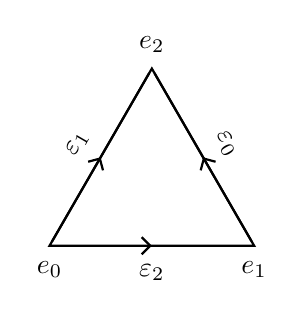
\begin{tikzpicture}[
      scale=1.5,
      decoration={markings,mark=at position 0.5 with {\arrow{Straight Barb[]}}},
      circ/.style={circle,minimum width=3pt,inner sep=0pt}
    ]
      \draw (-30:1) node [circ,label=-90:$e_1$] (e1) {} 
        -- (90:1) node [circ,label=90:$e_2$] (e2) {} 
        -- (210:1) node [circ,label=-90:$e_0$] (e0) {} -- cycle;
      \draw [postaction={decorate}] (e1) -- (e2) node [midway,sloped,above=3pt] {$\varepsilon_0$};
      \draw [postaction={decorate}] (e0) -- (e2) node [midway,sloped,above=3pt] {$\varepsilon_1$};
      \draw [postaction={decorate}] (e0) -- (e1) node [midway,sloped,below=3pt] {$\varepsilon_2$};
    \end{tikzpicture}
  \end{center}
  \begin{enumerate}
    \item 证明 $(\sigma_0*\sigma_1^-)*\sigma_2$ 相对于 $\partI$ 零伦。
    \item 证明 $(\sigma_1*\sigma_0^-)*\sigma_2^-$ 相对于 $\partI$ 零伦。
    \item 令 $F:I\times I\to X$ 是连续映射,按照上面的图定义 $X$ 中的
    道路 $\alpha,\beta,\gamma,\delta$。也即 $\alpha(t)=F(t,0)$,
    $\beta(t)=F(t,1)$,$\gamma(t)=F(0,t)$,$\delta(t)=F(1,t)$。
    证明 $\alpha\simeq \gamma *\beta *\delta^{-}\relhomo$。
  \end{enumerate}
\end{problem}
\begin{proof}
  (1) 考虑下图所示的同伦:
  \begin{center}
    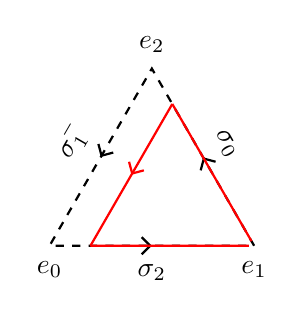
\begin{tikzpicture}[
      scale=1.5,
      decoration={markings,mark=at position 0.5 with {\arrow{Straight Barb[]}}},
      circ/.style={circle,minimum width=3pt,inner sep=0pt}
    ]
      \draw[dashed] (-30:1) node [circ,label=-90:$e_1$] (e1) {} 
      -- (90:1) node [circ,label=90:$e_2$] (e2) {} 
      -- (210:1) node [circ,label=-90:$e_0$] (e0) {} -- cycle;
      \draw [dashed,decorate] (e1) -- (e2) node [midway,sloped,above=3pt] {$\sigma_0$};
      \draw [dashed,decorate] (e2) -- (e0) node [midway,sloped,above=3pt] {$\sigma_1^-$};
      \draw [dashed,decorate] (e0) -- (e1) node [midway,sloped,below=3pt] {$\sigma_2$};
      \draw [red] (e1) -- ($(e1)!0.8!(e2)$);
      \draw [red,postaction=decorate] ($(e1)!0.8!(e2)$) -- ($(e1)!0.8!(e0)$);
      \draw [red] ($(e1)!0.8!(e0)$) -- (e1);
    \end{tikzpicture}
  \end{center}
  也即定义 $H:I\times I\to X$ 为
  \[
    H(s,t)=\begin{cases}
      \sigma\bigl((1-4s)e_1+4s\varepsilon_0(1-t)\bigr) & 0\leq s\leq \frac{1}{4},\\
      \sigma\bigl((2-4s)\varepsilon_0(1-t)+(4s-1)\varepsilon_2(t)\bigr)
      & \frac{1}{4}\leq s\leq \frac{1}{2},\\
      \sigma\bigl((2-2s)\varepsilon_2(t)+(2s-1)e_1\bigr) &
      \frac{1}{2}\leq s\leq 1.
    \end{cases}
  \]
  此时 $H$ 是 $(\sigma_0*\sigma_1^-)*\sigma_2$ 到 $e_1$ 的常值环道的相对同伦。

  (2) 与 (1) 同理。
\end{proof}

\begin{problem}{}{* is not a group}
  \begin{enumerate}
    \item (1) 如果 $f\simeq g\relhomo$,那么
    $f^-\simeq g^-\relhomo$。
    \item 如果道路 $f,g$ 满足 $\omega(f)=\alpha(g)$,那么
    \[
      (f*g)^{-}=g^-*f^-.
    \]
    \item 给出一个环道 $f$ 使得 $f*f^-\neq f^-*f$ 的例子。
    \item 如果 $\alpha(f)=p$ 且 $f$ 不是常值,那么 $i_p*f\neq f$。
  \end{enumerate}
\end{problem}
\begin{proof}
  (1) 设 $H:f\simeq g\relhomo$,定义 
  $ G(s,t)=H(1-s,t) $ 即可。

  (2) 我们有
  \[
    (f*g)^-(s)=f*g(1-s)=\begin{cases}
      g(1-2s) & 0\leq s\leq \frac{1}{2},\\
      f(2-2s) & \frac{1}{2}\leq s\leq 1.
    \end{cases}
  \]
  另一方面,有
  \[
    (g^-*f^-)(s)=\begin{cases}
      g^-(2s) & s\leq \frac{1}{2}\\
      f^-(2s-1) & s\geq \frac{1}{2}
    \end{cases}=\begin{cases}
      g(1-2s) & 0\leq s\leq \frac{1}{2},\\
      f(2-2s) & \frac{1}{2}\leq s\leq 1.
    \end{cases}.
  \]

  (3) 
\end{proof}

\ref{prob:* is not a group} 表明在道路乘法 $*$ 的作用下道路集合不能形成
一个群。但是下面的定理告诉我们对于道路类来说可以解决大部分问题。

\begin{theorem}\label{thm:groupoid}
  $X$ 是空间,那么 $X$ 的所有道路类集合在乘法 $[f][g]=[f*g]$ 下形成
  一个群胚,其满足下面的性质:
  \begin{enumerate}
    \item 每个道路类 $[f]$ 有一个起始点 $\alpha[f]=p\in X$ 
    以及终点 $\omega[f]=q\in X$,并且
    \[
      [i_p][f]=[f]=[f][i_q];
    \]
    \item 当道路乘法有意义的时候,结合律总是成立;
    \item 如果 $p=\alpha[f]$ 以及 $q=\omega[f]$,那么
    \[
      [f][f^-]=[i_p],\quad [f^-][f]=[i_q].
    \]
  \end{enumerate}
\end{theorem}
\begin{proof}
  (1) 我们证明 $i_p*f\simeq f\relhomo$ 即可。我们可以画出下面的图来理解。
  \begin{center}
    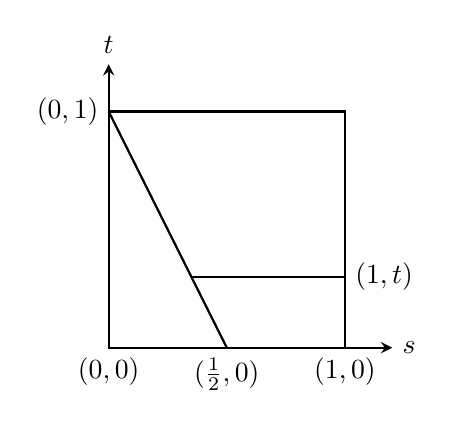
\begin{tikzpicture}[scale=3]
      \draw (0,0) coordinate(O) rectangle (1,1) coordinate(P);
      \draw[-stealth] (O) -- (1.2,0) node [right]{$s$};
      \draw[-stealth] (O) -- (0,1.2) node [above]{$t$};
      \node[below] at (O-|P) {$(1,0)$};
      \node[below] at (O) {$(0,0)$};
      \node[below] at ($(O)!0.5!(O-|P)$) {$(\frac{1}{2},0)$};
      \node[left] at (O|-P) {$(0,1)$};
      \draw[postaction=decorate] ($(O)!0.5!(O-|P)$) coordinate (S) -- (O|-P);
      \coordinate (T) at ($(S)!0.3!(O|-P)$);
      \draw (T) -- (T-|P) node[right] {$(1,t)$};
    \end{tikzpicture}
  \end{center}
  对于固定的 $t\in I$,我们需要一个仿射映射 $\theta_t:[(1-t)/2,1]\to [0,1]$,这样
  $f(\theta_t(s))$ 就是一个道路。根据 \ref{prob:affine expr},我们有
  \[
    \theta_t(s)=\frac{2}{1+t}s+\frac{t-1}{t+1}.
  \]
  于是定义 $H:I\times I\to X$ 为
  \[
    H(s,t)=\begin{cases}
      p & s\leq \frac{1-t}{2},\\
      f(\theta_t(s)) & s\geq \frac{1-t}{2},
    \end{cases}
  \]
  就有 $H:i_p*f\simeq f\relhomo$。对于 $[f][i_q]=[f]$ 类似。

  (2) 我们需要证明 $\bigl([f][g]\bigr)[h]=[f]\bigl([g][h]\bigr)$,即
  证明 $(f*g)*h\simeq f*(g*h)\relhomo$。
  画图可得
  \begin{center}
    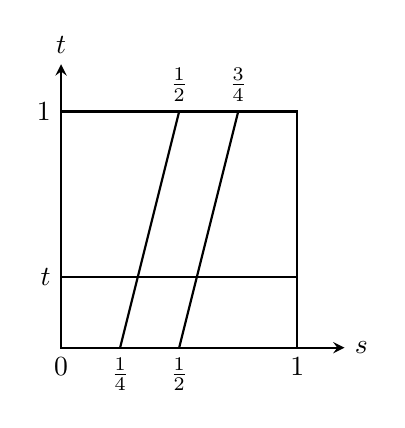
\begin{tikzpicture}[scale=3]
      \draw (0,0) coordinate(O) rectangle (1,1) coordinate(P);
      \draw[-stealth] (O) -- (1.2,0) node [right]{$s$};
      \draw[-stealth] (O) -- (0,1.2) node [above]{$t$};
      \node[below] at (O-|P) {$1$};
      \node[below] at (O) {$0$};
      \node[left] at (O|-P) {$1$};
      \coordinate[label={[below]$\frac{1}{2}$}] (1/2) at ($(O)!0.5!(O-|P)$); 
      \coordinate[label={[below]$\frac{1}{4}$}] (1/4) at ($(O)!0.25!(O-|P)$); 
      \coordinate[label={[above]$\frac{1}{2}$}] (1/2u) at ($(O|-P)!0.5!(P)$); 
      \coordinate[label={[above]$\frac{3}{4}$}] (3/4) at ($(O|-P)!0.75!(P)$); 
      \draw (1/4) -- (1/2u);
      \draw (1/2) -- (3/4);
      \draw (0,0.3) node[left]{$t$} -- (1,0.3);
    \end{tikzpicture}
  \end{center}
  令 $\theta_t:[0,(1+t)/4]\to [0,1]$,$\sigma_t:[(1+t)/4,(2+t)/4]\to [0,1]$,
  $\mu_t:[(2+t)/4,1]\to [0,1]$ 是仿射映射,那么
  \[
    H(s,t)=\begin{cases}
      f(\theta_t(s)) & s\leq \frac{1+t}{4},\\
      g(\sigma_t(s)) & \frac{1+t}{4}\leq s\leq\frac{2+t}{4},\\
      h(\mu_t(s)) & s\geq \frac{2+t}{4}
    \end{cases}
  \]
  即为所求的相对同伦。

  (3) 我们证明 $f*f^-\simeq i_p\relhomo$。画图可得
  \begin{center}
    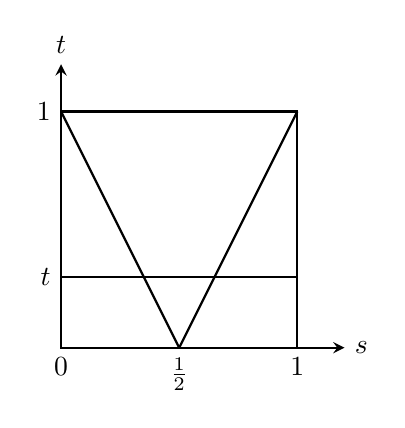
\begin{tikzpicture}[scale=3]
      \draw (0,0) coordinate(O) rectangle (1,1) coordinate(P);
      \draw[-stealth] (O) -- (1.2,0) node [right]{$s$};
      \draw[-stealth] (O) -- (0,1.2) node [above]{$t$};
      \node[below] at (O-|P) {$1$};
      \node[below] at (O) {$0$};
      \node[left] at (O|-P) {$1$};
      \coordinate[label={[below]$\frac{1}{2}$}] (1/2) at ($(O)!0.5!(O-|P)$); 
      \draw (1/2) -- (O|-P);
      \draw (1/2) -- (P);
      \draw (0,0.3) node[left]{$t$} -- (1,0.3);
    \end{tikzpicture}
  \end{center}
  令 $\theta_t:[0,(1-t)/2]\to [0,1]$,$\sigma_t:[(1-t)/2,(1+t)/2]\to [0,1]$,
  $\mu_t:[(1+t)/2,1]\to [0,1]$ 是仿射映射,那么
  \[
    H(s,t)=\begin{cases}
      f(\theta_t(s)) & s\leq \frac{1-t}{2},\\
      i_q(\sigma_t(s)) & \frac{1-t}{2}\leq s\leq\frac{1+t}{2},\\
      f^-(\mu_t(s)) & s\geq \frac{1+t}{2}
    \end{cases}
  \]
  即为所求的相对同伦。
\end{proof}

\autoref{thm:groupoid} 中的道路类并不构成群,因为道路类的乘法并不总是有定义。我们以最简单的
方式弥补这一点,即只关注环道。

\begin{definition}
  固定一个点 $x_0\in X$,这个点被称为\emph{基点}。定义 $X$ 在基点 $x_0$ 处的\emph{基本群}为
  \[
    \pi_1(X,x_0)=\bigl\{[f]\,|\,\alpha[f]=x_0=\omega[f]\bigr\}.
  \]
  群乘法为
  \[
    [f][g]=[f*g].
  \]
\end{definition}

根据 \autoref{thm:groupoid},我们知道 $\pi_1(X,x_0)$ 确实是一个群。


\section{函子 \texorpdfstring{$\pi_1$}{pi}}

我们已经引入了带点拓扑范畴 $\cat{Top_*}$,此时态射 $f:(X,x_0)\to (Y,y_0)$
是保持基点的连续映射 $f:X\to Y$,即 $f(x_0)=y_0$。在 $\cat{Top_*}$ 中,
我们通常选择 $0$ 作为 $I$ 的基点,$1$ 作为 $\mathbb{S}^1$ 的基点。

\begin{theorem}
  $\pi_1:\cat{Top_*}\to\cat{Grp}$ 是一个协变函子。此外,如果 $h,k:(X,x_0)\to (Y,y_0)$
  满足 $h\simeq k\rel\{x_0\}$,那么 $\pi_1(h)=\pi_1(k)$。
\end{theorem}
\begin{proof}
  如果 $[f]\in \pi_1(X,x_0)$,定义 $\pi_1(h):\pi_1(X,x_0)\to \pi_1(Y,y_0)$
  为 $[f]\mapsto [h\circ f]$。若 $f\simeq f'\relhomo$,
  那么 $h\circ f\simeq h\circ f'\relhomo$,所以 $\pi_1(h)$ 是良定义的。
  假设 $f,g$ 是 $x_0$ 处的两个环道,那么容易发现有
  \[
    h\circ (f*g)=(h\circ f)*(h\circ g),
  \]
  所以 $\pi_1(h)$ 是群同态。不难验证 $\pi_1$ 保持复合和恒等映射,
  所以 $\pi_1$ 是函子。

  若 $h\simeq k\rel\{x_0\}$,那么对于任意 $x_0$ 处的环道 $f$ 有 $h\circ f\simeq k\circ f\relhomo$,
  所以 $\pi_1(h)=\pi_1(k)$。
\end{proof}

\begin{remark}
  \begin{enumerate}
    \item 
    此后,我们通常使用 $h_*$ 来表示 $\pi_1(h)$,$h_*$ 被称为 $h$ 诱导的。
    \item 我们证明了当 $h\simeq k\rel\{x_0\}$ 的时候有 $h_*=k_*$,
    但是,如果 $h\simeq k$ 仅仅是自由同伦,那么不一定有 $h_*=k_*$。
    \item 实际上我们可以定义\emph{带点同伦范畴} $\cat{hTop_*}$,
    其作为相对同伦的共轭导出的商范畴。也就是说,$\cat{hTop_*}$
    的对象是带点拓扑空间 $(X,x_0)$,态射 $(X,x_0)\to (Y,y_0)$
    是相对同伦类 $[f]$,其中 $f:(X,x_0)\to (Y,y_0)$
    是带点映射。态射复合为 $[h][f]=[h\circ f]$。根据 
    \ref{prob:homotopy on S^1},每个环道 $f:I\to (Y,y_0)$
    都可以视为一个带点映射 $f':(\mathbb{S}^1,1)\to (Y,y_0)$。
    如果 $\cat{hTop_*}$ 的 $\Hom$ 集合记为 $[(X,x_0),(Y,y_0)]$,那么
    $[f]\to [f']$ 给出了一个双射
    \[
      \pi_1(Y,y_0)\to [(\mathbb{S}^1,1),(Y,y_0)].
    \]
    使用 \ref{prob:homotopy on S^1} 的 (2),我们可以在 $\Hom$ 集合
    上引入乘法,即 $[f'][g']=[(f*g)']$。此时这个双射就是一个同构。
    因此 $\pi_1$ 是一个协变 $\Hom$ 函子的例子。粗略地说,
    空间 $(Y,y_0)$ 的基本群仅仅是 $\cat{hTop_*}$ 中的态射 
    $(\mathbb{S}^1,1)\to (Y,y_0)$ 的集合。我们将在介绍更高阶的同伦群
    函子 $\pi_n$ 的时候使用这一点。
  \end{enumerate}  
\end{remark}

令 $x_0$ 是空间 $X$ 的一个基点,$A$ 是包含 $x_0$ 的一个子空间,包含映射
$\iota:(A,x_0)\to (X,x_0)$ 是带点映射,因此诱导了同态 $\iota_*:\pi_1(A,x_0)\to\pi_1(X,x_0)$,
即 $[f]\mapsto [\iota f]$。此时环道 $\iota f$ 仅仅是将 $f$ 视为 $X$ 
中的环道。此时可能出现下面的情况:$f$ 在 $A$ 中不是零伦的,但是 $f$ 
(准确的说是 $\iota f$)在 $X$ 中是零伦的。例如,取 $X$ 是包含 $A$ 的可缩空间
(比方说锥体 $CA$)。这意味着 $X$ 的额外空间可能允许 $f$ 收缩为 $X$ 中的一点。
所以,这意味着同态 $\iota_*$ 可能有非平凡的核。

\begin{theorem}
  令 $x_0\in X$,$X_0$ 是 $X$ 的包含 $x_0$ 的道路连通分支,那么
  \[
    \pi_1(X_0,x_0)\simeq \pi_1(X,x_0).
  \]
\end{theorem}
\begin{proof}
  令 $\iota:(X_0,x_0)\hookrightarrow (X,x_0)$ 是包含映射。如果 $[f]\in\ker\iota_*$,
  那么 $\iota f\simeq i_{x_0}\relhomo$。设 $F:I\times I\to X$ 是这样的同伦,
  那么 $F(0,0)=x_0$。由于 $F(I\times I)$ 道路连通并且 
  $x_0=F(0,0)\in F(I\times I)$,所以 $F(I\times I)\subseteq X_0$,
  这就表明 $F$ 可以视为到 $X_0$ 的连续映射,所以 $f$ 在 $X_0$ 中是零伦的,
  即 $\iota_*$ 是单射。下面任取环道 $f:I\to X$,同样的 $f(I)$
  是包含 $x_0$ 的道路连通集合,所以 $f(I)\subseteq X_0$,于是我们可以定义
  环道 $f':I\to X_0$ 为 $f'(s)=f(s)$,此时 $f=\iota f'$,即
  $[f]=[\iota f']=\iota_*[f']$,故 $\iota_*$ 是满射。
\end{proof}

那么当基点改变的时候会发生什么?

\begin{theorem}
  如果 $X$ 道路连通且 $x_0,x_1\in X$,那么
  \[
    \pi_1(X,x_0)\simeq \pi_1(X,x_1).
  \]
\end{theorem}
\begin{proof}
  设 $\gamma$ 是从 $x_0$ 到 $x_1$ 的道路。定义 $\varphi:\pi_1(X,x_0)\to\pi_1(X,x_1)$
  为 $[f]\mapsto [\gamma^-][f][\gamma]$。不难验证这是一个群同态且有
  逆映射 $[g]\mapsto [\gamma][g][\gamma^-]$。
\end{proof}

\begin{theorem}
  如果 $(X,x_0)$ 和 $(Y,y_0)$ 是带点空间,那么
  \[
    \pi_1\bigl(X\times Y,(x_0,y_0)\bigr)\simeq \pi_1(X,x_0)\times \pi_1(Y,y_0).
  \]
\end{theorem}
\begin{proof}
  令 $p:(X\times Y,(x_0,y_0))\to (X,x_0)$ 和 $q:(X\times Y,(x_0,y_0))\to (Y,y_0)$
  是投影映射。那么 $(p_*,q_*):[f]\mapsto \bigl([pf],[qf]\bigr)$
  是一个同态。设 $g$ 是 $x_0$ 处的环道,$h$ 是 $y_0$ 处的环道,那么
  $(g,h)(s)=(g(s),h(s))$ 是 $(x_0,y_0)$ 处的环道。定义 
  $\theta:\pi_1(X,x_0)\times \pi_1(Y,y_0)\to \pi_1\bigl(X\times Y,(x_0,y_0)\bigr)$
  为
  \[
    \theta\bigl([g],[h]\bigr)=[(g,h)],
  \]
  不难验证 $\theta$ 是良定义的,且和 $(p_*,q_*)$ 互逆。
\end{proof}

\begin{problem}{}{}
  给出一个不是局部道路连通的可缩空间的例子。
\end{problem}
\begin{solution}
  令 $X$ 是 $\sin(1/x)$ 空间,此时 $CX$ 可缩。考虑 $x=[(0,0),0]$
  处的一个邻域,这个邻域不包含顶点 $[(0,0),1]$。此时可以找到足够小的
  $\varepsilon$ 使得 $y=[(\varepsilon,\sin 1/\varepsilon),0]$
  在这个邻域中。此时 $x$ 到 $y$ 的任意道路都可以投影为
  从 $(0,0)$ 到 $(\varepsilon,\sin 1/\varepsilon)$ 的道路,这是不存在的。
  所以 $CX$ 不是局部道路连通的。
\end{solution}

\begin{problem}{}{}
  令 $X$ 是空间。证明存在一个范畴 $\cat C$ 满足 $\ob\cat C=X$,并且
  $\Hom(p,q)=\{[f]\,|\,\alpha[f]=p,\omega[f]=q\}$,复合
  $\Hom(p,q)\times \Hom(q,r)\to\Hom(p,r)$ 为
  $\bigl([f],[g]\bigr)\mapsto [f*g]$。证明 $\cat C$ 中的每个态射都是
  同构。
\end{problem}

接下来的问题是,具有相同同伦型的空间是否有同构的基本群?

\begin{lemma}\label{lemma:free homotopy}
  令 $\varphi_0,\varphi_1:X\to Y$ 是连续映射。
  假设 $F:\varphi_0\simeq\varphi_1$ 是(自由)同伦,选取 $x_0\in X$,
  令 $\lambda$ 是 $Y$ 中从 $\varphi_0(x_0)$ 到 $\varphi_1(x_0)$
  的道路 $F(x_0,\cdot )$。那么存在一个交换图
  \[
    \begin{tikzcd}[sep=large]
      \pi_1(X,x_0)\arrow[r,"\varphi_{1*}"]\arrow[dr,"\varphi_{0*}"'] & \pi_1\bigl(Y,\varphi_1(x_0)\bigr)
      \arrow[d,"\psi"]\\
      & \pi_1\bigl(Y,\varphi_0(x_0)\bigr),
    \end{tikzcd}
  \]
  其中 $\psi$ 是同构 $[g]\mapsto [\lambda*g*\lambda^-]$。
\end{lemma}
\begin{proof}
  任取 $[f]\in\pi_1(X,x_0)$,我们需要证明
  $\varphi_0\circ f\simeq \lambda*(\varphi_1\circ f)*\lambda^-\relhomo$。
  定义 $G:I\times I\to Y$ 为
  \[
    G(s,t)=F(f(s),t),
  \]
  那么 $G:\varphi_0\circ f\simeq \varphi_1\circ f$。当然,这里
  $\varphi_0\circ f$ 是 $\varphi_0(x_0)$ 处的环道,$\varphi_1\circ f$
  是 $\varphi_1(x_0)$ 处的环道。
\end{proof}

\begin{corollary}
  假设 $\varphi_i:(X,x_0)\to (Y,y_0)$ 是自由同伦的。
  \begin{enumerate}
    \item $\varphi_{0*}$ 和 $\varphi_{1*}$ 是共轭的:即
    存在 $[\lambda]\in\pi_1(Y,y_0)$ 使得 
    $\varphi_{0*}[f]=[\lambda]\varphi_{1*}\bigl([f]\bigr)[\lambda]^{-1}$。
    \item 如果 $\pi_1(Y,y_0)$ 是交换群,那么 $\varphi_{0*}=\varphi_{1*}$。
  \end{enumerate}
\end{corollary}
\begin{proof}
  我们有 $\varphi_0(x_0)=y_0=\varphi_1(x_0)$,此时 $\lambda$ 是 $y_0$
  处的环道,因此 $[\lambda]\in\pi_1(Y,y_0)$。根据引理,我们有
  \[ 
    [\varphi_0\circ f]=[\lambda*(\varphi_1\circ f)*\lambda^-].
  \]
  这就证明了 (1)。对于 (2),交换性表明可以先计算 $[\lambda][\lambda]^{-1}$,
  所以 $\varphi_{0*}=\varphi_{1*}$。
\end{proof}

\begin{theorem}
  如果 $\beta:X\to Y$ 是同伦等价,那么任取 $x_0\in X$,
  同态 $\beta_*:\pi_1(X,x_0)\to \pi_1(Y,y_0)$ 都是同构。
\end{theorem}
\begin{proof}
  设 $\alpha:Y\to X$ 使得 $\alpha\circ\beta\simeq 1_X$ 以及
  $\beta\circ \alpha\simeq 1_Y$。根据引理,我们有交换图
  \[
    \begin{tikzcd}[sep=large]
      & \pi_1(Y,\beta(x_0))\arrow[dr,"\alpha_*"] & \\
      \pi_1(X,x_0)\arrow[ur,"\beta_*"]\arrow[rr,"(\alpha\beta)_*"]
      \arrow[dr,"(1_X)_*"'] & &
      \pi_1(X,\alpha\beta(x_0))\arrow[dl,"\psi"]\\
      & \pi_1(X,x_0) & 
    \end{tikzcd}
  \]
  注意利用 $\pi_1$ 的函子性。因为 $\psi$ 是同构,所以 $(\alpha\beta)_*$ 是同构。
  这表明 $\beta_*$ 是单射。类似的,利用 $\beta\circ\alpha\simeq 1_Y$
  可以得出 $\beta_*$ 是满射,所以 $\beta_*$ 是同构。
\end{proof}

\begin{corollary}
  令 $X,Y$ 是有相同同伦型的道路连通空间,那么对于任意 $x_0\in X,y_0\in Y$,
  都有
  \[
    \pi_1(X,x_0)\simeq \pi_1(Y,y_0).
  \]
\end{corollary}
\begin{proof}
  上面的定理表明 $\pi_1(X,x_0)\simeq\pi_1(Y,\beta(x_0))$,
  其中 $\beta:X\to Y$ 是同伦等价。道路连通性表明基本群与基点的选取无关。
\end{proof}

\begin{corollary}
  如果 $X$ 是可缩的且 $x_0\in X$,那么
  \[
    \pi_1(X,x_0)=\{1\}.
  \]
\end{corollary}

\begin{definition}
  空间 $X$ 如果道路连通且对任意 $x_0\in X$ 有 $\pi_1(X,x_0)=\{1\}$,那么我们说
  $X$ 是\emph{单连通}的。
\end{definition}

注意有的作者允许单连通空间不道路连通,那么此时意味着每个道路连通分支
是本书意义下的单连通空间。

我们已经证明可缩空间是单连通的,但是反过来不一定正确。
例如,我们后面将会证明 $\mathbb{S}^n$ 在 $n\geq 2$ 的时候都是
单连通的,但是它们都不可缩。


\begin{corollary}
  如果 $\beta:(X,x_0)\to (Y,y_0)$ 是零伦的,那么诱导的
  同态 $\beta_*:\pi_1(X,x_0)\to \pi_1(Y,y_0)$ 是平凡的。
\end{corollary}
\begin{proof}
  令 $k:X\to Y$ 是 $y_1$ 处的常值映射,假设 $\beta\simeq k$。
  此时 $k_*:\pi_1(X,x_0)\to \pi_1(Y,y_1)$ 是平凡的,
  因为 $k_*[f]=[k\circ f]$ 是单位元。根据
  \autoref{lemma:free homotopy},存在同构 $\psi$
  使得 $\psi\beta_*=k_*$,所以 $\beta_*=\psi^{-1}k_*$
  是平凡的。
\end{proof}

\section{\texorpdfstring{$\pi_1(\mathbb{S}^1)$}{圆的基本群}}

因为 $\pi_1(X,x_0)$ 由所有映射 $\mathbb{S}^1\to X$ 的相对同伦类构成,
所以考虑 $X=\mathbb{S}^1$ 本身的时候是自然的。

\begin{lemma}\label{lemma:lift of X}
  令 $X$ 是 $\mathbb{R}^k$ 的一个紧凸集,$f:(X,x_0)\to (\mathbb{S}^1,1)$
  是连续映射,令 $t_0\in \mathbb{Z}$,那么存在唯一的连续映射
  $\tilde f:(X,x_0)\to (\mathbb{R},t_0)$ 使得 $\exp 2\pi i \tilde f=f$。
  \[
    \begin{tikzcd}[sep=large]
      & (\mathbb{R},t_0)\arrow[d,"\pi"] \\
      (X,x_0)\arrow[ur,"\tilde f",dashed]\arrow[r,"f"']
      & (\mathbb{S}^1,1).
    \end{tikzcd}
  \]
  其中 $\pi$ 表示 $\pi(x)=\exp 2\pi i x$。
\end{lemma}
\begin{remark}
  \begin{enumerate}
    \item $\tilde{f}$ 被称为 $f$ 的\emph{提升}。
    \item 为了满足 $\exp 2\pi i \tilde f(x_0)=f(x_0)=1$,
    $t_0$ 必须是整数。
  \end{enumerate}
\end{remark}
\begin{proof}
  思路是将 $\pi$ 限制在 $(-\frac{1}{2},\frac{1}{2})$ 上,此时 $\pi$ 是到 $\mathbb{S}^1 \smallsetminus\{-1\}$
  是同胚映射,我们直接考虑其逆映射 $\lambda$。此时我们自然地想定义 $\tilde f(x)=t_0+\lambda(f(x))$,
  因为这使得 $\tilde f(x_0)=t_0+\lambda(1)=t_0$。但是问题在于可能存在 $f(x)=-1$ 的情况,所以我们需要
  做一点技术性的处理。
  
  因为 $X$ 是紧的,所以 $f$ 一致连续,所以存在 $\varepsilon>0$ 使得 $\norm{x-x'}<\varepsilon$ 的时候有
  $\norm{f(x)-f(x')}<2$,这里选取 $2$ 是因为这保证 $f(x),f(x')$ 不会是对径点。$X$
  有界表明存在 $n$ 使得 $\norm{x-x_0}/n<\varepsilon$。

  对于每个 $x\in X$,我们连接 $x_0$ 到 $x$ 的线段,$X$ 的凸性保证了这仍然在 $X$ 中。将这个线段 $n$ 等分,
  设等分点为 $x_0,x_1,\dots,x_n=x$。那么 $\norm{x_j-x_{j+1}}=\norm{x-x_0}/n<\varepsilon$,所以
  $f(x_j)$ 和 $f(x_{j+1})$ 不会是对径点,也即 $f(x_j)^{-1}f(x_{j+1})\neq -1$。
  这就表明 $f(x_j)^{-1}f(x_{j+1})\in \mathbb{S}^1 \smallsetminus\{-1\}$。注意到
  \[
    f(x)=f(x_0)\bigl[f(x_0)^{-1}f(x_1)\bigr]\bigl[f(x_1)^{-1}f(x_2)\bigr]\cdots\bigl[f(x_{n-1})^{-1}f(x_n)\bigr],
  \]
  所以我们定义 $g_j:X\to \mathbb{S}^1 \smallsetminus\{-1\}$ 为
  $g_j(x)=f(x_j)^{-1}f(x_{j+1})$,所以
  \[
    f(x)=f(x_0)g_0(x)g_1(x)\cdots g_{n-1}(x).
  \]
  于是我们定义 $\tilde{f}:X\to \mathbb{R}$ 为
  \[
    \tilde{f}(x)=t_0+\lambda(g_0(x))+\lambda_1(g_1(x))+\cdots+\lambda(g_{n-1}(x)),
  \]
  此时便有 $\tilde{f}(x_0)=t_0$。

  下面证明唯一性即可。假设 $\tilde g:X\to \mathbb{R}$ 也是满足上述交换图的带点连续映射。定义
  $h:X\to \mathbb{R}$ 为 $h(x)=\tilde{f}(x)-\tilde{g}(x)$。此时
  \[
    \pi h(x)=\pi\bigl(\tilde{f}(x)-\tilde{g}(x)\bigr)=\pi \tilde{f}(x)/\pi \tilde{g}(x)=1,
  \]
  所以 $h$ 的取值一定是整数,又因为 $X$ 是连通的,所以 $h$ 一定是常值的且值为某个整数。
  而 $h(x_0)=\tilde{f}(x_0)-\tilde{g}(x_0)=t_0-t_0=0$,所以 $\tilde{f}=\tilde{g}$。
\end{proof}

\begin{corollary}\label{coro:lift of path}
  令 $f:(I,\partI)\to (\mathbb{S}^1,1)$ 是连续映射。
  \begin{enumerate}
    \item 存在唯一的连续映射 $\tilde{f}:I\to \mathbb{R}$ 使得 $\exp 2\pi i \tilde{f}=f$
    并且 $\tilde{f}(0)=0$。
    \item 如果 $g:(I,\partI)\to (\mathbb{S}^1,1)$ 是连续映射并且 $f\simeq g\relhomo$,
    那么 $\tilde{f}\simeq \tilde{g}\relhomo$,此外 $\tilde{f}(1)=\tilde{g}(1)$。
  \end{enumerate}
\end{corollary}
\begin{proof}
  (1) 利用上面的引理即得。

  (2) 设 $F:I\times I\to \mathbb{S}^1$ 是相对同伦,于是 $F(0,0)=f(0)=1$。引理表明存在连续映射 $\wtilde F:I\times I\to \mathbb{R}$
  使得 $\wtilde F(0,0)=0$ 且 $\exp 2\pi i \wtilde F=F$。我们证明 $\wtilde F:\tilde f\simeq \tilde g\relhomo$。

  考虑 $\varphi_0(s)=\wtilde F(s,0)$,那么  $\exp 2\pi i\varphi_0(s)=\exp 2\pi i\wtilde F(s,0)=F(s,0)=f(s)$,
  根据提升的唯一性,所以 $\varphi_0=\tilde f$。类似的,可以证明 $\wtilde F(s,1)=\tilde g$。
  下面我们还要说明 $\wtilde F$ 是相对同伦。考虑 $\theta_0(t)=\wtilde F(0,t)$,
  那么 $\exp 2\pi i \theta_0(t)=F(0,t)=1$,结合 $\theta_0(0)=0$,所以
  $\theta_0(t)=0$。类似的可以证明 $\wtilde F(1,t)=0$。这就表明 $\wtilde F:\tilde f\simeq \tilde g\relhomo$。
  此外,还有 $\tilde f(1)=\wtilde F(1,t)=g(1)$。
\end{proof}

直观上来说,这意味着如果 $f,g$ 相对同伦,那么它们的提升的终点一定相同,也即“缠绕的圈数”一定相同。

\begin{definition}
  如果 $f:(I,\partI)\to (\mathbb{S}^1,1)$ 是连续映射,定义 $f$ 的\emph{映射度}为
  \[
    \deg f=\tilde f(1),
  \]
  其中 $\tilde f$ 是 $f$ 的唯一满足 $\tilde f(0)=0$ 的提升。
\end{definition}

注意到 $\exp 2\pi i \tilde f(1)=f(1)=1$,所以 $\deg f$ 一定是整数。

\begin{theorem}
  定义函数 $d:\pi_1(\mathbb{S}^1,1)\to \mathbb{Z}$ 为 $[f]\mapsto \deg f$,这是一个群同构。
  特别地,有 $\deg (f*g)=\deg f+\deg g$。
\end{theorem}
\begin{proof}
  \autoref{coro:lift of path} 告诉我们 $d$ 是良好定义的。然后我们说明 $d$ 是满射。
  对于任意 $m\in \mathbb{Z}$,函数 $f(s)=\exp 2\pi i ms$ 有映射度 $m$,
  所以 $d$ 是满射。现在先假设 $d$ 是同态,说明 $d$ 是单射。令 $\deg f=0$,那么
  $f$ 的提升满足 $\tilde f(1)=0$,于是 $\tilde f$ 是 $\mathbb{R}$ 中以 $0$ 为基点的环道。
  现在 $\pi:(\mathbb{R},0)\to (\mathbb{S}^1,1)$ 诱导出群同态 $\pi_1(\mathbb{R},0)\to \pi_1(\mathbb{S}^1,1)$
  使得 $[\tilde f]\mapsto [\pi\circ \tilde f]=[f]$,$\mathbb{R}$ 可缩表明 $\pi_1(\mathbb{R},0)$
  是平凡群,所以 $[f]=1$ 是 $\pi_1(\mathbb{S}^1,1)$ 的单位元,故 $d$ 是单射。
  
  现在只需要说明 $d$ 是群同态。假设 $f,g$ 分别是 $\mathbb{S}^1$ 中以 $1$ 为基点的映射度为
  $m,n$ 的环道。我们需要计算 $\deg(f*g)$,也即寻找道路 $\tilde h:I\to \mathbb{R}$ 使得
  $\exp 2\pi i \tilde h=f*g$ 且 $\tilde h(0)=0$。设 $\tilde g$ 是 $g$ 的提升且 $\tilde g(0)=0$,
  定义 $\tilde \gamma:I\to \mathbb{R}$ 是 $\tilde{\gamma}(s)=m+\tilde g(s)$,此时
  $\tilde{\gamma}$ 是从 $m$ 到 $m+n$ 的道路。令 $\tilde f$ 是 $f$ 的提升且 $\tilde f(0)=0$,
  那么 $\tilde f*\tilde \gamma$ 有意义(因为 $\tilde f(1)=\deg f=m$)且 
  $\tilde f*\tilde \gamma(0)=0$,$\tilde f*\tilde \gamma(1)=m+n$。我们断言
  $\tilde{f}*\tilde{\gamma}$ 是 $f*g$ 的提升即可。这只需要直接验证:
  \[
    \exp\bigl(2\pi i(\tilde f*\tilde \gamma)(s)\bigr)=\begin{cases}
      f(2s) & 0\leq s\leq \frac{1}{2},\\
      g(2s-1) & \frac{1}{2}\leq s\leq 1.
    \end{cases}
  \]
  这就说明了 $d$ 是群同构。
\end{proof}

\begin{corollary}
  $\mathbb{S}^1$ 不是单连通的。
\end{corollary}

\begin{corollary}
  $\mathbb{S}^1$ 中的两个以 $1$ 为基点的环道相对同伦当且仅当它们有相同的映射度。
\end{corollary}
\begin{proof}
  如果 $f\simeq g\relhomo$,根据 \autoref{coro:lift of path},就有 $\deg f=\deg g$。
  反之,若 $\deg f=\deg g$,那么 $[f]=[g]$。
\end{proof}


\begin{definition}
  一个\emph{拓扑群}指的是群 $G$ 同时是一个拓扑空间,满足:
  \begin{enumerate}
    \item 乘法映射 $\mu:G\times G\to G$ 是连续映射;
    \item 逆映射 $i:G\to G$ 是连续映射。
  \end{enumerate}
\end{definition}

\begin{definition}
  对于一个带点空间 $(X,x_0)$,如果存在一个带点映射
  $m:\bigl(X\times X,(x_0,x_0)\bigr)\to (X,x_0)$ 使得 $(X,x_0)$ 上的带点映射
  $m(x_0,\cdot)$ 和 $m(\cdot,x_0)$ 都相对 $\{x_0\}$ 同伦于 $1_X$,那么
  我们说 $(X,x_0)$ 是\emph{$H$-空间},$x_0$ 是\emph{同伦单位元}。
\end{definition}

显然,任意拓扑群 $X$ 带上单位元 $x_0$ 和群乘法 $m$ 都是 $H$-空间。

如果 $k:X\to X$ 是 $x_0$ 处的常值映射,记 $(k,1_X):X\to X\times X$
是映射 $x\mapsto (x_0,x)$,那么 $m(x_0,\cdot)=m\circ (k,1_X)$。
同理,有 $m(\cdot,x_0)=m\circ (1_X,k)$。

\begin{theorem}
  如果 $(X,x_0)$ 是 $H$-空间,那么 $\pi_1(X,x_0)$ 是交换群。
\end{theorem}
\begin{proof}
  我们已经证明了 $\theta:\pi_1(X,x_0)\times\pi_1(X,x_0)\to\pi_1\bigl(X\times X,(x_0,x_0)\bigr)$
  是同构映射,满足 $\bigl([f],[g]\bigr)\mapsto [(f,g)]$。
  任取 $[f],[g]\in\pi_1(X,x_0)$,那么我们有
  \begin{align*}
    [g]&=[1_X\circ g]=[m(x_0,\cdot)\circ g]=\bigl(m\circ (k,1_X)\bigr)_*[g]
    \\
    &=m_*(k,1_X)_*[g]=m_*[(kg,g)]=m_*\theta\bigl([kg],[g]\bigr)\\
    &=m_*\theta(e,[g]).
  \end{align*}
  其中 $e=[kg]$ 是 $\pi_1(X,x_0)$ 的单位元。类似的,还有
  \[
    [f]=m_*\theta([f],e).
  \]
  因为 $m_*\theta$ 是群同态,所以
  \begin{align*}
    m_*\theta\bigl([f],[g]\bigr)&=m_*\theta\bigl((e,[g])([f],e)\bigr)\\
    &=m_*\theta(e,[g])m_*\theta([f],e)=[g][f],
  \end{align*}
  另一方面利用 $([f],[g])=([f],e)(e,[g])$,可以得出
  $m_*\theta\bigl([f],[g]\bigr)=[f][g]$,所以
  $[f][g]=[g][f]$,即 $\pi_1(X,x_0)$ 是交换群。
\end{proof}

\begin{corollary}
  如果 $G$ 是拓扑群,那么 $\pi_1(G,e)$ 是交换群。
\end{corollary}

上述推论的逆否命题更有趣。如果 $X$ 是拓扑空间,但是 $\pi_1(X,x_0)$
不交换,这意味着无法在 $X$ 上定义一个群结构使得其成为一个拓扑群。

\chapter{奇异同调}

\section{奇异复形和同调函子}

\begin{definition}
  $\Delta^n=[e_0,e_1,\dots,e_n]$ 的一个\emph{定向}指的是一组有序的顶点。
\end{definition}

\begin{definition}
  $\Delta^n$ 的两个定向是\emph{相同的},如果它们作为
  $\{e_0,e_1,\dots,e_n\}$ 上的置换有相同的奇偶性。否则
  说它们是\emph{相反的}。
\end{definition}

给定一个 $\Delta^n$ 的定向,可以诱导出其 $i$-面上的定向,即
$(-1)^i[e_0,\dots,\hat e_i,\dots,e_n]$。例如,假设 $\Delta^2$
被逆时针定向:
\begin{center}
  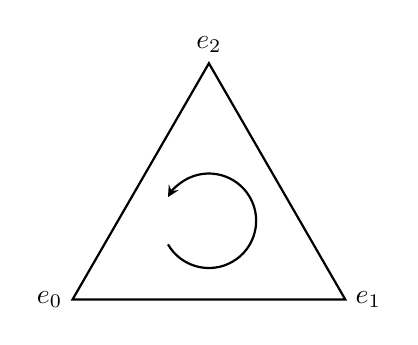
\begin{tikzpicture}[scale=2]
    \draw (-30:1) node [right] {$e_1$} -- (90:1) node[above]{$e_2$} -- (210:1) node[left]{$e_0$} -- cycle;
    \draw[-stealth] (-150:0.3) arc(-150:150:0.3);
  \end{tikzpicture} 
\end{center}
那么 $\Delta^2$ 的 $0$-面是 $[\hat e_0,e_1,e_2]=[e_1,e_2]$,定向为
$[e_1,e_2]$。$1$-面是 $[e_0,\hat e_1,e_2]=[e_0,e_2]$,定向为
$-[e_0,e_2]=[e_2,e_0]$。$2$-面是 $[e_0,e_1,\hat e_2]=[e_0,e_1]$,
定向为 $[e_0,e_1]$。

于是 $\Delta^2$ 的边界为 
\[
  [\hat e_0,e_1,e_2]\cup [e_0,\hat e_1,e_2]\cup [e_0,e_1,\hat e_2],
\]
定向边界为
\[
  [\hat e_0,e_1,e_2]\cup -[e_0,\hat e_1,e_2]\cup [e_0,e_1,\hat e_2].
\]
一般的,可以定义 $\Delta^n=[e_0,e_1,\dots,e_n]$ 的边界为
$\bigcup_{i=0}^n [e_0,\dots,\hat e_i,\dots,e_n]$,
定向边界为 $\bigcup_{i=0}^n (-1)^i[e_0,\dots,\hat e_i,\dots,e_n]$。

\begin{definition}
  令 $X$ 是拓扑空间,$X$ 中的一个\emph{(奇异)$n$-单纯形}指的是
  连续映射 $\sigma:\Delta^n\to X$,其中 $\Delta^n$ 是标准 $n$-单纯形。
\end{definition}

因为 $\Delta^1$ 就是闭区间,所以 $X$ 中的奇异 1-单纯形本质上就是 $X$
中的一个道路。因为 $\Delta^0$ 是单点集,所以奇异 0-单纯形被视为 $X$
中的一个点。

\begin{definition}
  令 $X$ 是拓扑空间,对于每个 $n\geq 0$,定义 $S_n(X)$
  是以 $X$ 中的奇异 $n$-单纯形为基生成的自由 Abelian 群。
  定义 $S_{-1}(X)=0$。$S_n(X)$ 的元素被称为 $X$
  中的\emph{(奇异)$n$-链}。
\end{definition}

一个奇异 $n$-单纯形 $\sigma:\Delta^n\to X$ 的定向边界应该为
$\sum_{i=0}^n(-1)^i\sigma|_{[e_0,\dots,\hat e_i,\dots,e_n]}$,
但是 $[e_0,\dots,\hat e_i,\dots,e_n]$ 不是标准 $(n-1)$-单纯形 $\Delta^{n-1}$。
不过我们可以通过一些简单的技巧弥补这一点。对于每个 $n$ 和 $i$,定义
$i$-面映射
\[
  \varepsilon_i^n:\Delta^{n-1}\to \Delta^n 
\]
为将 $\Delta^{n-1}$ 的顶点 $\{e_0,\dots,e_{n-1}\}$ 送到 $\Delta^n$
的顶点 $\{e_0,\dots,\hat e_i,\dots,e_n\}$ 的仿射映射,并且其保持
坐标的顺序:
\begin{align*}
  &\varepsilon_0^n:(t_0,\dots,t_{n-1})\mapsto (0,t_0,\dots,t_{n-1});\\
  &\varepsilon_in:(t_0,\dots,t_{n-1})\mapsto (t_0,\dots,t_{i-1},0,t_{i+1},\dots,t_{n-1}).
\end{align*}
例如,面映射 $\varepsilon_i^2:\Delta^1\to \Delta^2$ 满足
$\varepsilon_0^2:[e_0,e_1]\mapsto [e_1,e_2]$,
$\varepsilon_1^2:[e_0,e_1]\mapsto [e_0,e_2]$,
$\varepsilon_2^2:[e_0,e_1]\mapsto [e_0,e_1]$。
注意上述例子中左右两端的 $e_i$ 表示的含义是不同的。

\begin{definition}
  如果 $\sigma:\Delta^n\to X$ 是连续映射并且 $n>0$,定义\emph{边界}为
  \[
    \partial_n\sigma=\sum_{i=0}^n (-1)^i\sigma\varepsilon_i^n\in S_{n-1}(X).
  \]
  如果 $n=0$,定义 $\partial_0\sigma=0$。
\end{definition}

注意到当 $X=\Delta^n$ 且 $\delta:\Delta^n\to\Delta^n$ 是恒等映射的时候,
有
\[
  \partial_n\delta=\sum_{i=0}^{n} (-1)^i\varepsilon_i^n,
\]
这和定向边界的定义是一致的。

\begin{theorem}
  对于每个 $n\geq 0$,存在唯一的同态 $\partial_n:S_n(X)\to S_{n-1}(X)$
  使得对于任意奇异 $n$-单纯形 $\sigma$ 有 
  $\partial_n\sigma=\sum_{i=0}^n(-1)^i\sigma\varepsilon_i^n$ 成立。
\end{theorem}

同态 $\partial_n:S_n(X)\to S_{n-1}(X)$ 被称为\emph{边界算子}。
对于空间 $X$,我们构造了一系列自由 Abelian 群和同态
\[
  \begin{tikzcd}
    \cdots\arrow[r] & S_n(X)\arrow[r,"\partial_n"] & S_{n-1}(X)
    \arrow[r] & \cdots\arrow[r] & S_1(X)\arrow[r,"\partial_1"]
    & S_0(X)\arrow[r,"\partial_0"] & 0.
  \end{tikzcd}
\]
这个链被称为 $X$ 的\emph{奇异复形},记为 $(S_*(X),\partial)$,
或者简记为 $S_*(X)$。

\begin{lemma}
  如果 $k<j$,那么面映射满足
  \[
    \varepsilon_j^{n+1}\varepsilon_k^n=\varepsilon_k^{n+1}\varepsilon_{j-1}^n
    :\Delta^{n-1}\to\Delta^{n+1}.
  \]
\end{lemma}

\begin{theorem}
  对于所有 $n\ge 0$,我们有 $\partial_n\circ \partial_{n+1}=0$。
\end{theorem}
\begin{proof}
  只需要对 $(n+1)$-单纯形 $\sigma$ 证明结论成立即可。根据上面的引理,我们有
  \begin{align*}
    \partial_n\partial_{n+1}\sigma&=
    \partial_n\left(\sum_j(-1)^j\sigma\varepsilon_j^{n+1}\right)\\
    &=\sum_{j,k}(-1)^{j+k}\sigma\varepsilon_j^{n+1}\varepsilon_k^n\\
    &=\sum_{j\leq k}(-1)^{j+k}\sigma\varepsilon_j^{n+1}\varepsilon_k^n
    +\sum_{k<j} (-1)^{j+k}\sigma\varepsilon_j^{n+1}\varepsilon_k^n\\
    &=\sum_{j\le k}(-1)^{j+k}\sigma\varepsilon_j^{n+1}\varepsilon_k^n
    +\sum_{k<j} (-1)^{j+k}\sigma\varepsilon_k^{n+1}\varepsilon_{j-1}^n\\
    &=\sum_{j\le k}(-1)^{j+k}\sigma\varepsilon_j^{n+1}\varepsilon_k^n
    +\sum_{p\leq q}(-1)^{p+q-1}\sigma\varepsilon_p^{n+1}\varepsilon_q^n\\
    &=0.\qedhere
  \end{align*}
\end{proof}

\begin{definition}
  对于空间 $X$,记 $Z_n(X)=\ker\partial_n$,被称为\emph{(奇异)$n$-圈}。
  记 $B_n(X)=\im\partial_{n+1}$,被称为\emph{(奇异)$n$-边界}。
\end{definition}

\begin{corollary}
  对于空间 $X$ 和每个 $n\geq 0$,有
  \[
    B_n(X)\subseteq Z_n(X).
  \]
\end{corollary}

\begin{definition}
  对于每个 $n\geq 0$,定义 $X$ 的 $n$-阶\emph{(奇异)同调群}为
  \[
    H_n(X)=\frac{Z_n(X)}{B_n(X)}=\frac{\ker\partial_n}{\im\partial_{n+1}}.
  \]
  陪集 $z_n+B_n(X)$ 被称为 $z_n$ 的\emph{同调类},记为 $\cls z_n$。
\end{definition}

我们的下一个目的是证明 $H_n$ 实际上是一个函子 $\cat{Top}\to\cat{Ab}$。
如果 $f:X\to Y$ 是连续映射,$\sigma:\Delta^n\to X$ 是 $n$-单纯形,
那么 $f\circ \sigma:\Delta^n\to Y$ 是 $Y$ 中的 $n$-单纯形。
根据线性性可以拓展为一个同态 $f_\#:S_n(X)\to S_n(Y)$
为
\[
  f_\#\bigl(\sum m_\sigma\sigma\bigr)=\sum m_\sigma (f\circ\sigma),
  \quad m_\sigma\in \mathbb{Z}.
\]

\begin{lemma}
  如果 $f:X\to Y$ 连续,那么 $\partial_n f_\#=f_\#\partial_n$,
  也即有下面的交换图
  \[
    \begin{tikzcd}[sep=large]
     S_n(X)\arrow[r,"\partial_n"]\arrow[d,"f_\#"']
     & S_{n-1}(X)\arrow[d,"f_\#"] \\
     S_n(Y)\arrow[r,"\partial_n"] & S_{n-1}(Y). 
    \end{tikzcd}
  \]
\end{lemma}
\begin{proof}
  只需要对 $S_n(X)$ 的生成元 $\sigma$ 证明即可。我们有
  \[
    \partial_n f_\#(\sigma)=\partial_n(f\circ\sigma)
    =\sum (-1)^i f\circ\sigma \circ\varepsilon_i^{n},
  \]
  另一方面,有
  \[
    f_\#\partial_n(\sigma)=f_\#\left(\sum(-1)^i\sigma\varepsilon_i^n\right)
    =\sum (-1)^i f\circ\sigma\circ\varepsilon_i^n.\qedhere
  \]
\end{proof}

\begin{lemma}\label{lemma:f sharp}
  如果 $f:X\to Y$ 是连续映射,那么
  \[
    f_\#(Z_n(X))\subseteq Z_n(Y),\quad 
    f_\#(B_n(X))\subseteq B_n(Y).
  \]
\end{lemma}
\begin{proof}
  任取 $\alpha\in Z_n(X)$,那么 $\partial_n\alpha=0$,所以
  $\partial_n(f_\#\alpha)=f_\#(\partial_n\alpha)=f_\#(0)=0$,
  所以 $f_\#(\alpha)\in Z_n(Y)$。
  任取 $\beta\in B_n(X)$,那么存在 $\gamma\in S_{n+1}(X)$
  使得 $\beta=\partial_{n+1}\gamma$,所以
  $f_\#(\beta)=f_\#(\partial_{n+1}\gamma)=\partial_{n+1}(f_\#\gamma)$,
  故 $f_{\#}(\beta)\in\im\partial_{n+1}=B_n(Y)$。
\end{proof}

\begin{theorem}
  $H_n:\cat{Top}\to\cat{Ab}$ 是函子。
\end{theorem}
\begin{proof}
  如果 $f:X\to Y$ 是连续映射,定义
  \[
    H_n(f):H_n(X)\to H_n(Y)
  \]
  为 $z_n+B_n(X)\mapsto f_\# (z_n)+B_n(Y)$。

  \autoref{lemma:f sharp} 表明 $H_n(f)$ 是良定义的,即
  $f_\#(z_n)$ 确实在 $Z_n(Y)$ 中并且不依赖于代表元的选取。
  现在只需要逐条验证 $H_n(f)$ 是同态,保持态射复合和单位元即可,
  这只需要按照定义验证。
\end{proof}

\begin{corollary}
  如果 $X,Y$ 同胚,那么 $H_n(X)\simeq H_n(Y)$。
\end{corollary}

所以每个同调群 $H_n(X)$ 都是空间 $X$ 的一个拓扑不变量。
这也表明 $\rank H_n(X)$ 是 $X$ 的拓扑不变量。

\begin{definition}
  对于每个 $n\geq 0$,$\rank H_n(X)$ 被称为 $X$ 的 $n$ 
  阶 \emph{Betti 数}。
\end{definition}

\section{维数公理和紧支}

我们在上面利用\emph{奇异理论}定义了同调群,优点在于对于任意
拓扑空间都可以定义同调群。但是这种理论的缺点在于通常很难计算
特定空间 $X$ 的同调群 $H_n(X)$。如果我们仅仅将注意力限制在
多面体或者 CW 复形(稍后定义)上,那么针对 $H_n(X)$ 有其他的
定义方式(单纯理论和胞腔理论),此时计算 $H_n(X)$ 会更加容易。

\begin{theorem}[维数公理]
  如果 $X$ 是单点空间,那么对于所有 $n\geq 1$ 都有 $H_n(X)=0$。
\end{theorem}
\begin{proof}
  对于每个 $n\geq 0$,此时只有一个奇异 $n$-单纯形 $\sigma_n:\Delta^n\to X$,
  因此 $S_n(X)=\langle \sigma_n\rangle$ 是循环群。那么
  \[
    \partial_n\sigma_n=\sum_{i=0}^i(-1)^n\sigma_n\varepsilon_i^n
    =\sum_{i=0}^n (-1)^i \sigma_{n-1},
  \]
  最后一个等号是因为 $\sigma_n\varepsilon_i^n$ 是 $(n-1)$-单纯形,
  所以必须等于 $\sigma_{n-1}$。这表明 
  \[
    \partial_n\sigma_n=\begin{cases}
      0 & \text{$n$ is odd}\\
      \sigma_{n-1} & \text{$n$ is even}.
    \end{cases}
  \]
  所以 $n$ 是奇数的时候 $\partial_n=0$,$n$ 是偶数的时候 $\partial_n$
  是同构。当 $n>0$ 的时候,考虑链
  \[
    \begin{tikzcd}
      S_{n+1}(X)\arrow[r,"\partial_{n+1}"] & S_n(X)
      \arrow[r,"\partial_n"] & S_{n-1}(X).
    \end{tikzcd}
  \]
  如果 $n$ 是奇数,那么 $S_n(X)=\ker\partial_n=Z_n(X)$
  并且 $\partial_{n+1}$ 是同构,所以 $S_n(X)=\im\partial_{n+1}=\ker\partial_n$,
  即 $H_n(X)=0$。如果 $n$ 是偶数,那么 $\partial_n$ 是同构且
  $\im\partial_{n+1}=0$,所以 $\ker\partial_n=0=\im\partial_{n+1}$,即
  $H_n(X)=0$。
\end{proof}

\begin{definition}
  空间 $X$ 被称为\emph{无环的},如果对于所有的 $n\ge 1$,
  有 $H_n(X)=0$。
\end{definition}

\begin{problem}{}{}
  如果 $X=\emptyset$,证明对于所有的 $n\geq 0$ 有 $H_n(X)=0$。
\end{problem}
\begin{proof}
  此时不存在奇异 $n$-单纯形 $\sigma:\Delta^n\to X$,所以
  $S_n(X)=0$ 是平凡群。所以 $H_n(X)=0$。
\end{proof}

\begin{problem}{}{}
  如果 $X$ 是单点空间,那么 $H_0(X)\simeq \mathbb{Z}$。
\end{problem}
\begin{proof}
  此时 $H_0(X)=S_0(X)/B_0(X)$。由于 $\partial_1=0$,所以
  $B_0(X)=0$,所以 $H_0(X)=S_0(X)$ 是无限阶循环群,即
  同构于 $\mathbb{Z}$。
\end{proof}

\begin{problem}{}{}
  对于每个 $n\geq 0$,证明 $S_n:\cat{Top}\to \cat{Ab}$ 是函子。
\end{problem}
\begin{proof}
  定义 $S_n(f)=f_\#$。直接验证 $S_n$ 的函子性即可。
\end{proof}

\begin{theorem}\label{thm:H0 of component}
  如果 $\{X_\lambda\}$ 是 $X$ 的道路连通分支集合,那么对于每个
  $n\geq 0$,我们有
  \[
    H_n(X)\simeq \bigoplus_\lambda H_n(X_\lambda).
  \]
\end{theorem}
\begin{proof}
  如果 $\gamma=\sum m_i\sigma_i\in S_n(X)$,那么每个 $\im\sigma_i$
  都被 $X$ 的某个唯一的道路连通分支包含,设 $\gamma=\sum \gamma_\lambda$,
  其中每个 $\gamma_\lambda$ 表示一些组成 $\gamma$ 的满足 $\im\sigma_i\subseteq X_\lambda$ 
  的 $m_i\sigma_i$ 之和。不难发现映射 $\gamma\mapsto (\gamma_\lambda)$
  是同构 $S_n(X)\to \bigoplus_\gamma S_n(X_\gamma)$。
  现在我们说明 $\gamma$ 是圈当且仅每个 $\gamma_\lambda$ 是圈:因为
  $\partial_n\gamma_\lambda\in S_{n-1}(X_\lambda)$,所以 $\partial_n\gamma=\sum\partial_n\gamma_\lambda=0$
  当且仅当每个 $\partial_n\gamma_\lambda=0$。
  定义映射 $\theta_n:H_n(X)\to \bigoplus_\lambda H_n(X_\lambda)$ 为
  $\gamma+B_n(X)\mapsto \bigl(\gamma_\lambda+B_n(X_\lambda)\bigr)$,
  上面的叙述表明 $\theta_n$ 是良定义的并且是单射。$\theta_n$ 显然是满射,
  所以 $\theta_n$ 是同构。
\end{proof}

\begin{problem}{}{}
  计算 $H_n(\mathbb{S}^0)$。
\end{problem}
\begin{solution}
  $H_n(\mathbb{S}^0)=H_n(\{-1,1\})\simeq \mathbb{Z}\oplus \mathbb{Z}$。
\end{solution}

当然,即使在 $X$ 道路连通的情况下,计算 $H_n(X)$ 通常也是困难的。
但是,我们总是可以计算 $H_0(X)$。

\begin{theorem}\label{thm:H0 of space}
  \mbox{}
  \begin{enumerate}
    \item 如果 $X$ 是非空道路连通空间,那么 $H_0(X)\simeq \mathbb{Z}$。
    此外,如果 $x_0,x_1\in X$,那么 $x_0+B_0(X)=x_1+B_0(X)$ 
    是 $H_0(X)$ 的生成元。
    \item 对于任意空间 $X$,群 $H_0(X)$ 是秩 $\card\Lambda$ 的自由
    Abelian 群,其中 $\{X_\lambda\}_{\lambda\in \Lambda}$
    是道路连通分支族。
    \item 如果 $X,Y$ 道路连通并且 $f:X\to Y$ 是连续的,那么
    $f_*:H_0(X)\to H_0(Y)$ 把 $H_0(X)$ 的生成元送到 $H_0(Y)$ 的生成元。
  \end{enumerate}
\end{theorem}
\begin{proof}
  (1) 考虑奇异复形的末端
  \[
    \begin{tikzcd}
      S_1(X)\arrow[r,"\partial_1"] & S_0(X)\arrow[r,"\partial_0"] & 0,
    \end{tikzcd}
  \]
  此时 $H_0(X)=Z_0(X)/B_0(X)=S_0(X)/B_0(X)$。
  要证明 $H_0(X)\simeq \mathbb{Z}$,我们构造一个
  核为 $B_0(X)$ 的满同态 $S_0(X)\to \mathbb{Z}$ 即可。
  任取 $\gamma=\sum m_xx\in S_0(X)$,注意只有有限个 $m_x$ 不为零。
  定义同态 $\theta:S_0(X)\to \mathbb{Z}$ 为
  \[
    \theta(\gamma)=\sum m_x.
  \]
  不难发现这是一个满同态。我们只需要说明
  \[
    B_0(X)=\left\{\gamma\in S_0(X)\,\middle|\, \sum m_x=0\right\}
  \]
  即可。

  首先假设 $\gamma=\sum_i m_i x_i$ 使得 $\sum m_i=0$。任取 $x\in X$,
  设 $\sigma_i$ 是 $x$ 到 $x_i$ 的道路。注意到 $\partial_1\sigma_i=\sigma_i(e_1)-\sigma_i(e_0)=x_i-x$。
  现在考虑 $\sum m_i\sigma_i\in S_1(X)$,那么 
  \[
    \partial_1\bigl(\sum m_i\sigma_i\bigr)
    =\sum m_i\partial_1\sigma_i=\sum m_i(x_i-x)=
    \sum m_ix_i-\bigl(\sum m_i\bigr)x=\gamma,
  \]
  所以 $\gamma\in B_0(X)$。反之,设 $\gamma\in B_0(X)$,那么
  存在 $\sum n_i\tau_i$ 使得 $\gamma=\partial_1\bigl(\sum n_i\tau_i\bigr)$,
  即
  \[
    \gamma=\sum n_i\bigl(\tau_i(e_1)-\tau_i(e_0)\bigr)=
    \sum_i n_i\tau_i(e_1)-\sum_i n_i\tau_i(e_0),
  \]
  所以 $\gamma$ 的系数之和为零。

  令 $x_0,x_1\in X$。设 $\sigma$ 是从 $x_0$ 到 $x_1$ 的道路,
  那么 $x_0-x_1=\partial_1\sigma\in B_0(X)$,所以
  $x_0+B_0(X)=x_1+B_0(X)$。如果 $\gamma=\sum m_ix_i$ 给出 $H_0(X)$
  的生成元 $\gamma+B_0(X)$,那么 $\theta(\gamma)=\sum m_i=\pm 1$。通过给 $\gamma$
  添加负号,不妨设 $\sum m_i=1$。此时 $\gamma-x_0$ 的系数之和为零,
  所以 $\gamma-x_0\in B_0(X)$,所以 $x_0+B_0(X)=\gamma+B_0(X)$ 是生成元。

  (2) 根据 (1) 和 \autoref{thm:H0 of component} 即得。

  (3) 由 (1) 即得。
\end{proof}

我们可以比较函子 $\pi_0$ 和 $H_0$:$\pi_0(X)$ 是 $X$ 的道路连通分支的集合,
$H_0(X)$ 是一些 $\mathbb{Z}$ 的直和,直和取遍道路连通分支的个数。
这两个函子实际上捕捉了相同的信息,即道路连通分支的个数。

\begin{lemma}
  若 $A$ 是 $X$ 的子空间,包含映射 $\iota:A\hookrightarrow X$,那么
  对于任意 $n\geq 0$,$\iota_\#:S_n(A)\to S_n(X)$ 是单射。
\end{lemma}
\begin{proof}
  设 $\gamma=\sum m_i\sigma_i\in S_n(A)$ 使得 $\iota_\#(\gamma)=0$,
  那么 $\sum m_i(\iota\circ\sigma_i)=0$,这就表明 $m_i=0$,
  即 $\gamma=0$,所以 $\iota_\#$ 是单射。
\end{proof}

注意上述引理经常被使用,但是我们不会再显式地引用它。

\begin{definition}
  如果 $\zeta=\sum m_i\sigma_i\in S_n(X)$,那么定义 $\zeta$ 的
  \emph{支集} 为 $\supp\zeta=\bigcup \sigma_i(\Delta^n)$。
\end{definition}

显然 $\supp\zeta$ 是 $X$ 的紧子集,因为 $\supp\zeta$ 是紧集的有限并。

\begin{theorem}
  如果 $\zeta+B_n(X)\in H_n(X)$,那么存在 $X$ 的紧子集 $A$ 使得
  $\zeta+B_n(X)\in\im\iota_*$,其中 $\iota:A\hookrightarrow X$ 是包含映射。
\end{theorem}

\section{同伦公理}

我们的下一个目标是证明当 $f,g$ 同伦的时候对于所有的 $n$
有 $H_n(f)=H_n(g)$。

\begin{theorem}
  如果 $X$ 是 Euclid 空间的有界凸集,那么对于所有 $n\geq 1$ 有 $H_n(X)=0$。
  特别的,对于所有 $n\geq 1$ 和 $k$ 有 $H_n(D^k)=0$。
\end{theorem}
\begin{remark}
  如果 $X\neq\emptyset$,\autoref{thm:H0 of space} 表明 $H_0(X)=\mathbb{Z}$。
\end{remark}
\begin{proof}
  选取点 $b\in X$。对于每个 $n$-单纯形 $\sigma:\Delta^n\to X$,回顾
  问题 \ref{prob:cone of simplex},$\Delta^{n+1}$ 可以视为 $\Delta^n$
  的一个锥体,于是我们考虑“以 $b$ 为顶点的 $\sigma$ 的锥体”。定义
  $(n+1)$-单纯形 $\sigma_b:\Delta^{n+1}\to X$ 为
  \[
    \sigma_b(t_0,t_1,\dots,t_{n+1})=\begin{dcases}
      b & \text{if $t_0=1$},\\
      t_0b+(1-t_0)\sigma\left(
        \frac{t_1}{1-t_0},\dots,\frac{t_{n+1}}{1-t_0}
      \right) & \text{if $t_0\neq 1$}.
    \end{dcases}
  \]

  定义 $c_n:S_n(X)\to S_{n+1}(X)$ 为 $c_n(\sigma)=\sigma_b$,然后线性
  延拓为群同态。我们断言,对于 $n\geq 1$,有
  \begin{equation}\label{eq:boundary of cn}
    \partial_{n+1}c_n(\sigma)=\sigma-c_{n-1}\partial_n(\sigma).
  \end{equation}  
  如果我们忽略符号,这就是在说 $\sigma$ 上的锥体是 $\sigma$ 和
  $\sigma$ 的边界上的锥体的并。我们可以以 $\sigma$ 为 $2$-单纯形的情况
  为例:
  \begin{center}
    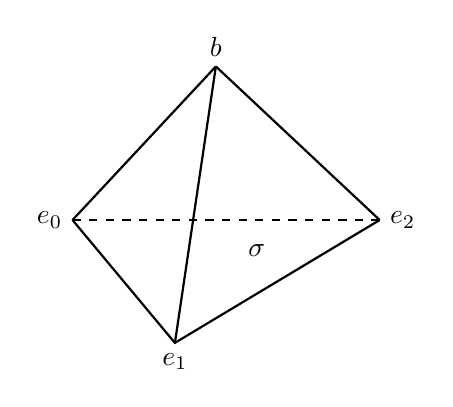
\begin{tikzpicture}[scale=1.3]
      \draw [dashed] (0,0) coordinate [label=180:$e_0$] (e0) --
        node[pos=0.6,below=5pt]{$\sigma$}
        (3,0)
        coordinate [label=0:$e_2$] (e2);
      \draw (e2)  -- (1,-1.2) coordinate[label=-90:$e_1$] (e1) -- (e0);
      \draw (1.4,1.5) coordinate[label=90:$b$](b) -- (e0);
      \draw (b) -- (e1);
      \draw (b) -- (e2);
    \end{tikzpicture}
  \end{center}
  这里 $\sigma$ 是 $[e_0,e_1,e_2]$,$\sigma_b$ 是整个三棱锥。此时
  $\sigma_b$ 的边界恰好为 $\sigma$ 以及三个面 $[b,e_0,e_1]$,
  $[b,e_0,e_2]$ 和 $[b,e_1,e_2]$,其中每个面都是 $\sigma$ 的边界上的锥体。

  如果 \eqref{eq:boundary of cn} 成立,那么定理的结论是显然的。因为对于任意
  $\gamma\in S_n(X)$,那么根据线性性有
  \[
    \gamma=\partial_{n+1}c_n\gamma+c_{n-1}\partial_n\gamma,
  \]
  于是 $\gamma\in Z_n(X)$ 表明 $\gamma=\partial_{n+1}c_n\gamma\in B_n(X)$,
  所以 $Z_n(X)=B_n(X)$,所以 $H_n(X)=0$。

  下面我们证明 \eqref{eq:boundary of cn} 式。首先计算
  $\sigma_b$ 的面映射,我们有
  \[
    (\sigma_b\varepsilon_0^{n+1})(t_0,\dots,t_{n})
    =\sigma_b(0,t_0,\dots,t_n)=\sigma(t_0,\dots,t_n),
  \]
  以及 $1\leq i\leq n+1$ 时有
  \[
    (\sigma_b\varepsilon_i^{n+1})(t_0,\dots,t_n)=
    \sigma_b(t_0,\dots,t_{i-1},0,t_{i+1},\dots,t_n).
  \]
  如果 $t_0=1$,那么 $\sigma_b(1,0,\dots,0)=b$。如果 $t_0\neq 1$,那么
  上式右端为
  \begin{align*}
    &t_0b+(1-t_0)\sigma\left(\frac{t_1}{1-t_0},\dots,\frac{t_{i-1}}{1-t_0},0,\frac{t_i}{1-t_0},\dots,\frac{t_n}{1-t_0}\right)\\
    &=t_0b+(1-t_0)\sigma\varepsilon_{i-1}^n\left(\frac{t_1}{1-t_0},\dots,\frac{t_n}{1-t_0}\right)\\
    &=c_{n-1}(\sigma\varepsilon_{i-1}^n)(t_0,\dots,t_n).
  \end{align*}
  所以
  \begin{align*}
    \partial_{n+1}c_n\sigma&=\sum_{i=0}^{n+1}(-1)^i (c_n\sigma)\varepsilon_i^{n+1}
    =\sigma+\sum_{i=1}^{n+1}(-1)^ic_{n-1}(\sigma\varepsilon_{i-1}^n)\\
    &=\sigma-\sum_{i=0}^n(-1)^ic_{n-1}(\sigma\varepsilon_i^n)\\
    &=\sigma-c_{n-1}\partial_n\sigma.\qedhere
  \end{align*}
\end{proof}






\end{document}
